\documentclass[type = bachelor]{whu-thesis}
\usepackage{textcomp,mathcomp}
\usepackage{siunitx}
\usepackage{chemfig}
\usepackage{graphicx}

\whusetup
  {
    info               =
      {
        title          = {金刚石氮-空位色心的\\电荷态调控和性质表征},
        title*         = {Modulation of Charge States and Characterization of Properties\\ in Nitrogen-Vacancy Centers of Diamond},
        student-number = {2020302192129},
        school         = {弘毅学堂},
        author         = {邹迪玮},
        author*        = {Diwei Zou},
        subject        = {学科},
        major          = {微电子科学与工程},
        advisor        = {周\ \ \ \ 利, 副教授;孙启超, 研究员},
        direction      = {研究方向},
        date           = {2024/5},
        keywords       = {关键词 1 , 关键词 2 , 关键词 3 , 关键词 4 , 一个非常非常,非常非常长——的关键词 5},
        keywords*      = {key word 1 , key word 2 , key word 3 , key word 4 , {and a very very, very very long key word---the key word 5}},
      },
    style              =
      {
        graphics-path  = {{figures/}{data/}},
        list-of-figures,
        list-of-tables,
      },
    element            =
      {
        innovation     = {pages/innovation},
        abstract       = {pages/abstract},
        abstract*      = {pages/enabstract},
        bibliography   = {ref/refs}
      }
  }
\begin{document}

% Chapter 5

\chapter{结果与讨论}

\section{曲线的模拟和仿真分析}

我们根据第二章中的公式利用$Python$进行了曲线的模拟和仿真分析,分别分析了不同读出时间$t_r$、不同的594 nm橙光激光功率对概率分布和过程参数($\gamma_0$, $\gamma_-$, $g_{0-}$, $g_{-0}$)的影响。除此之外,还探究了不同的过程参数对概率分布的影响。在这个过程中,通过对模拟数据的数值仿真,我们可以更好地理解和估算实验数据的特征,为实验结果的解释提供更多的参考。

\subsection{不同读出时间$t_r$对概率分布的影响}
我们探究了不同读出时间$t_r$对概率分布的影响,在同样的参数下,改变读出时间$t_r$,得到了图 \ref{fig: tR_variation}中的概率分布曲线。
\begin{figure}
  \centering
  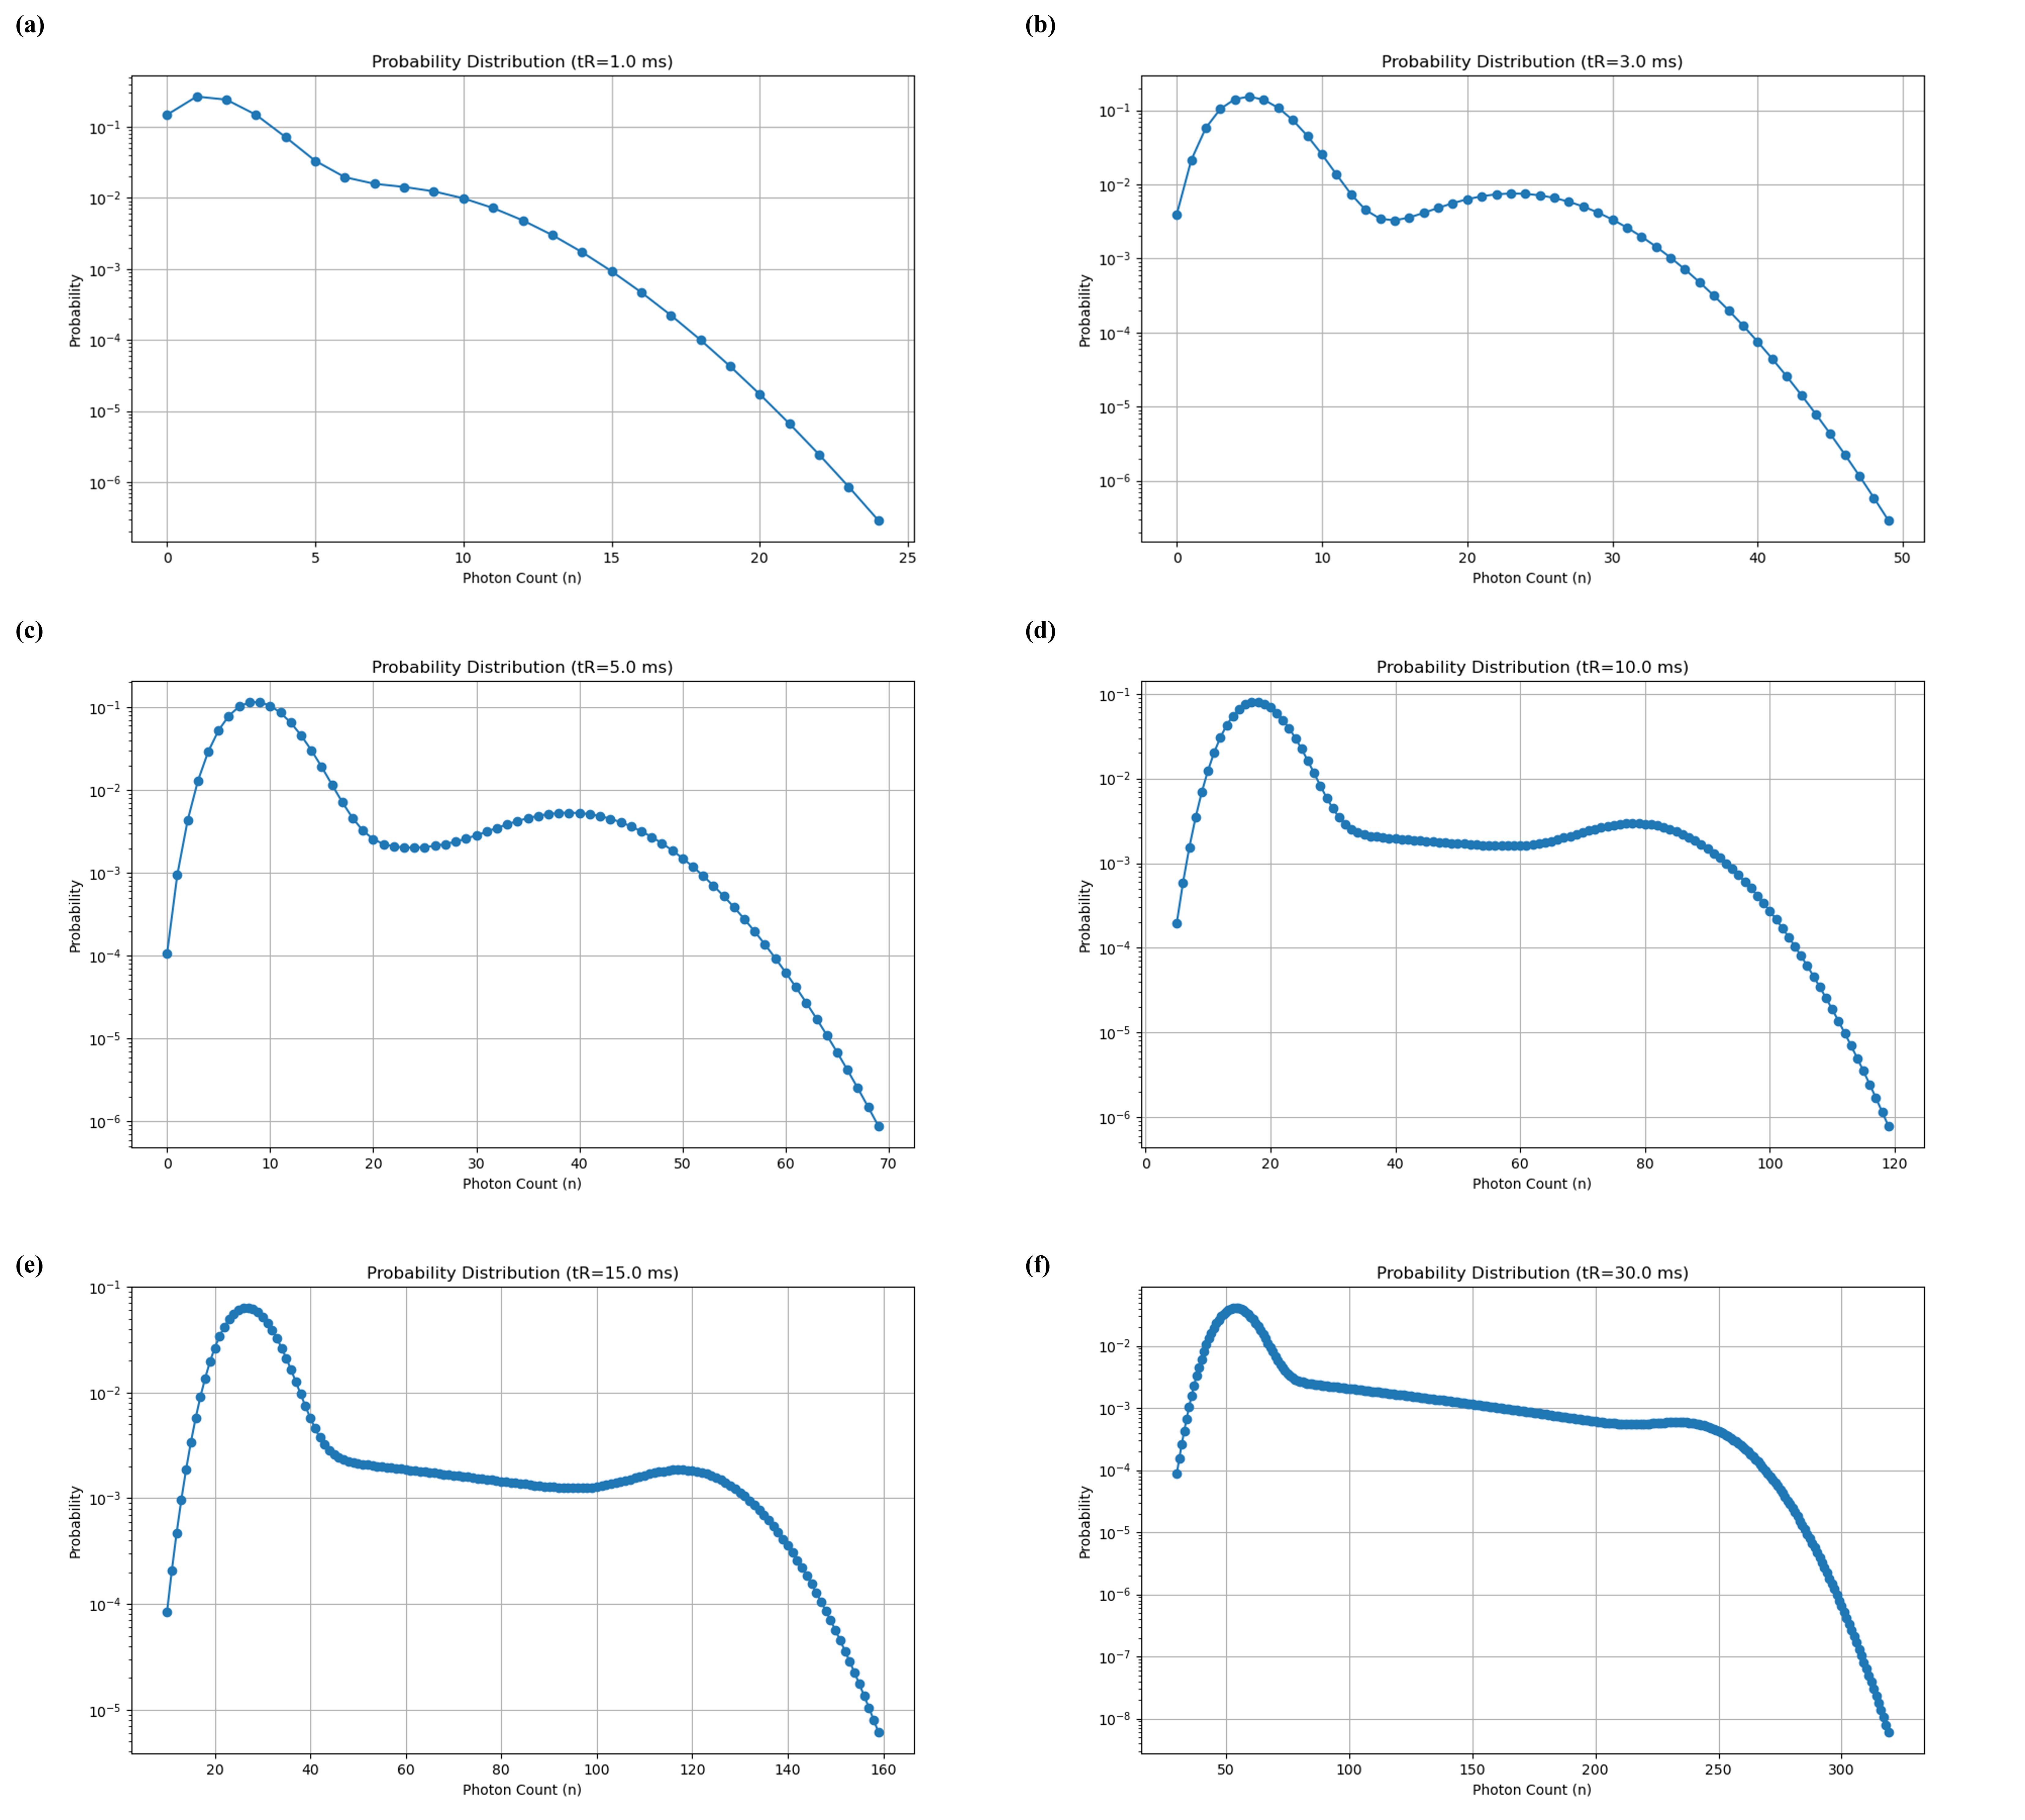
\includegraphics[width=1.0\textwidth]{figures/Chapter 5/tR_variation.png}
  \caption[不同的读出时间$t_r$下的概率分布曲线]{不同的读出时间$t_r$下的概率分布曲线,图中的“tR”表示读出时间$t_r$,分别为1.0 ms、3.0 ms、5.0 ms、10.0 ms、15.0 ms和30.0 ms。横轴代表着每个读出时间$t_r$内出现的光子数Photon Count (n),纵轴表示读取到n个光子的情况所出现的概率,以对数坐标表示。}
  \label{fig: tR_variation}
\end{figure}
在这个过程中,我们设置NV$^0$的低计数率为$\gamma_0$ = 1803 pcs/s,NV$^-$的高计数率为$\gamma_-$ = 8090 pcs/s,NV$^0$到NV$^-$的结合速率$g_{0-}$ = 66.0 s$^{-1}$,NV$^-$到NV$^0$的电离速率$g_{-0}$ = 7.3 s$^{-1}$。显然,由于APD前的长通滤波片的存在,结合NV$^-$和NV$^0$的光谱性质,可以显而易见地预见$\gamma_0 < \gamma_- $。

从图 \ref{fig: tR_variation}中可以看到,随着读出时间$t_r$的增加,横轴的数据整体增大,即随着$t_r$(time bin)的变宽,每个time bin中所出现的光子数整体上更多。曲线整体呈现中间高,两边低的趋势,也就是说不论$t_r$的长度是多少,都可能出现光子数较多或者光子数较少的情况,但是发生的概率比较低。
\begin{figure}
  \centering
  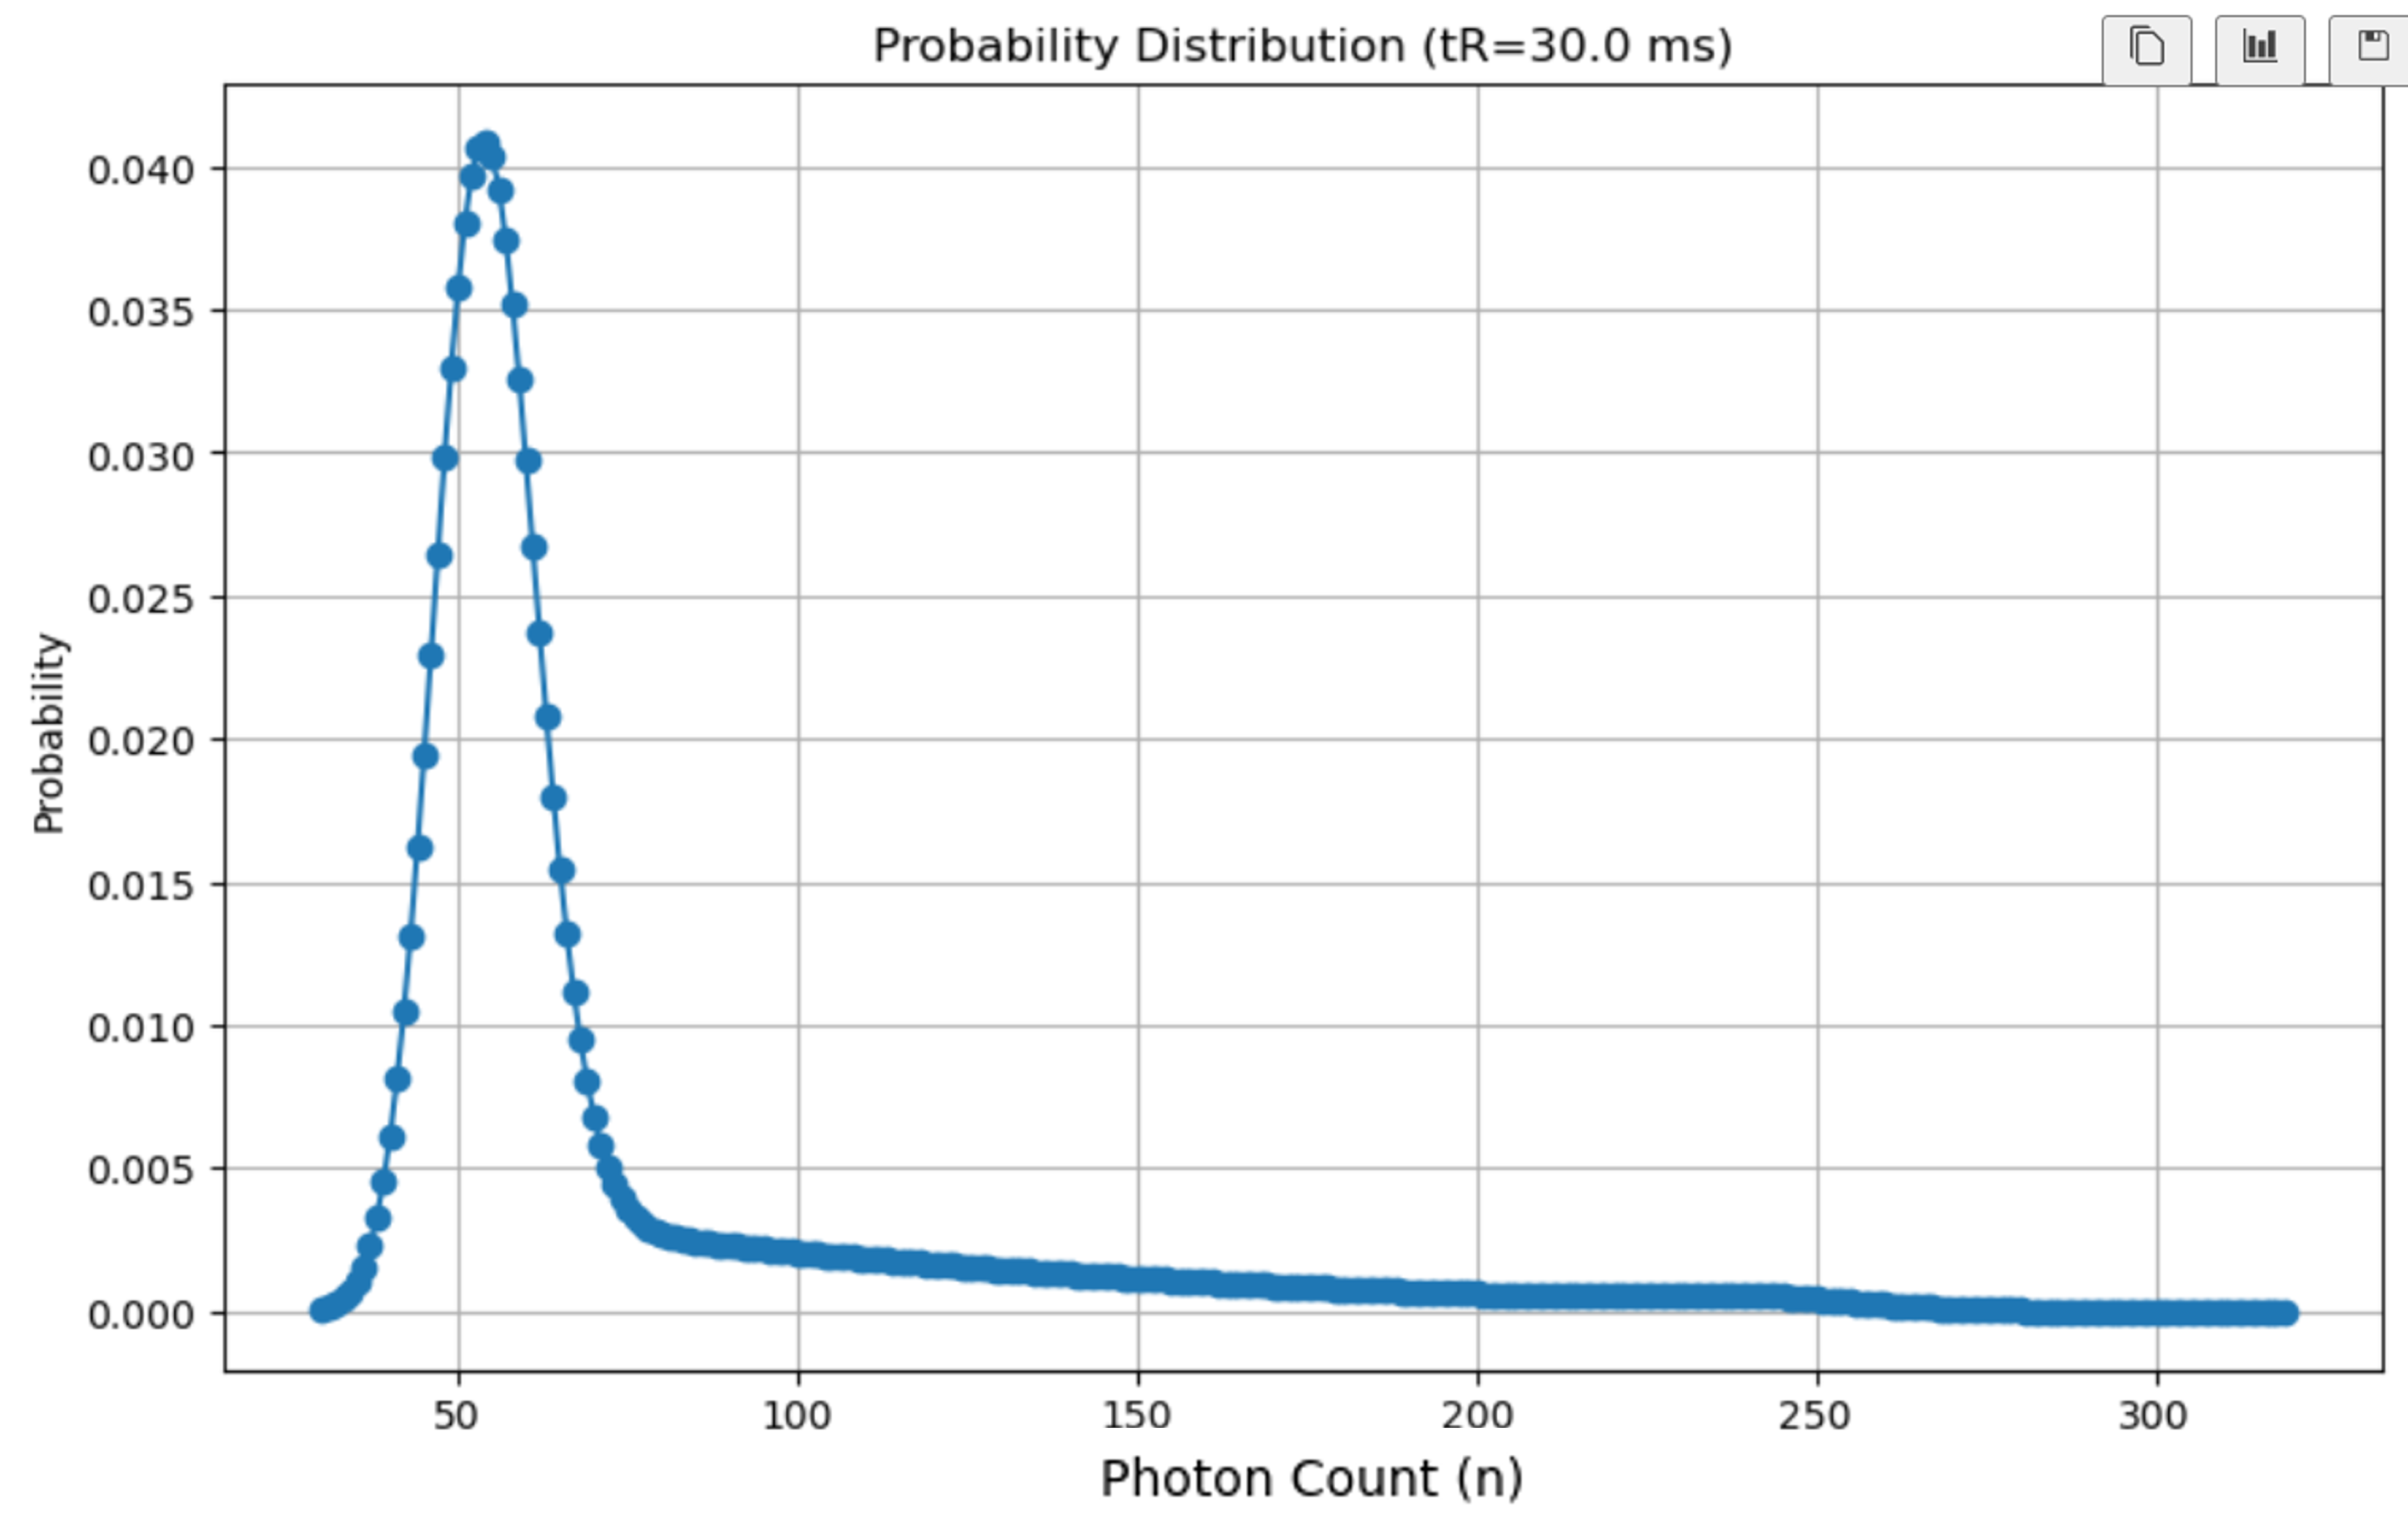
\includegraphics[width=0.8\textwidth]{figures/Chapter 5/tR_isometric.png}
  \caption[等间距纵轴概率坐标在$t_r$ = 30.0 ms时的概率分布图]{等间距纵轴概率坐标在$t_r$ = 30.0 ms时的概率分布图。}
  \label{fig: tR_isometric}
\end{figure}
因为概率分布比较集中,如果用常规的等间距纵轴概率坐标的话,曲线会呈现图 \ref{fig: tR_isometric}所示的状态,因此用对数坐标会呈现出两个峰值的结果,便于分析和观测。对比不同$t_r$下的概率分布曲线,我们可以看到,随着$t_r$的增加,两个峰值的位置和高度都有所变化,两个峰值之间的距离分隔也就越远,拟合的准确性就更好。这是由于NV$^0$和NV$^-$的计数率差距较大,读出时间越长,两者的光子数差异也就越大,因此两个峰值之间的距离也就越大。然而,$t_r$也并不是越大越好,在$t_r$过大的情况下,数据整体的分辨率会下降,所以要选取合适的$t_r$来得到最好的拟合效果。除此之外,无论$t_r$选取什么样的值,左右两侧都有概率较小的情况发生,这些概率较小的部分可以忽略,在实际实验中基本不可能发生,因此在拟合的过程中,除了图 \ref{fig: tR_variation}(f)外,其余都选择了只显示概率为10$^{-6}$附近或者更高的部分;对于图 \ref{fig: tR_variation}(f)而言,我们选择了更广的范围以获得更完整的曲线形态,从而便于同其他$t_r$的情况的概率分布曲线进行比较和分析。

\subsection{不同读出光强$P_{594}$对概率分布的影响}

在分析完不同的读出时间$t_r$对于电荷态分布情况的影响后,我们进一步探究了不同的读出光强$P_{594}$对概率分布的影响。根据$Shields$等人的文章,我们可以通过下列式子来计算不同的594 nm的激光功率对NV$^0$和NV$^-$的影响 \cite{Shields2015}:
\begin{equation}
  \gamma_0(P)=\frac{\alpha_0 P}{1+\frac{P}{P_{Sat,0}}}+C_{dark}
  \label{equ: gamma_0}
\end{equation}
\begin{equation}
  \gamma_-(P)=\frac{\alpha_- P}{1+\frac{P}{P_{Sat,-}}}+C_{dark}
  \label{equ: gamma_-}
\end{equation}
考虑到光强对于单NV Center的激发是一个单光子过程,NV Center可以被看成一个单光子源,所以NV$^0$和NV$^-$的计数率和激发功率类似于光强饱和曲线的形式。其中$\alpha$为一个比例系数,$P_{Sat}$是饱和而光强,装置系统整体的暗计数为$C_{dark} = 950\ s^{-1}$。根据相似的思路,NV$^0$和NV$^-$之间的相互转换(电离和复合)率,可以用以下的式子计算:
\begin{equation}
  g_{0-} = \frac{\beta_{0-}P^2}{1+\frac{P}{P_{Sat,0}}}
  \label{equ: g_0-}
\end{equation}
\begin{equation}
  g_{-0} = \frac{\beta_{-0}P^2}{1+\frac{P}{P_{Sat,-}}}
  \label{equ: g_-0}
\end{equation}
根据之前的实验结果,可以其系数参数为\cite{Robledo2011}:

$\alpha_0 = 1901 \pm 45\ (\mu W \cdot s)^{-1}$

$\alpha_- = 15384 \pm 310\ (\mu W \cdot s)^{-1}$

$P_{Sat,0} = 120 \pm 13\ (\mu W)$

$P_{Sat,-} = 54 \pm 7\ (\mu W)$

$\beta_{0-} = 30 \pm 1\ (\mu W)^{-2} \cdot s^{-1}$

$\beta_{-0} = 208 \pm 8\ (\mu W)^{-2} \cdot s^{-1}$

值得注意的是,这里的参数是利用Nano-pillars结构所测试得到的,所以饱和光强相较于直接在表面注入的色心所得到的结果要低一些,也就是说Nano-pillars结构能提高激发和收集效率,使其中的NV Center在较低光强的情况下就能轻松达到荧光发光饱和的状态。四个相关的参数$\gamma_0$、$\gamma_-$、$g_{0-}$和$g_{-0}$随着读出的594 nm橙光激光功率的变化如图 \ref{fig: P_variation_parameters}所示。
\begin{figure}
  \centering
  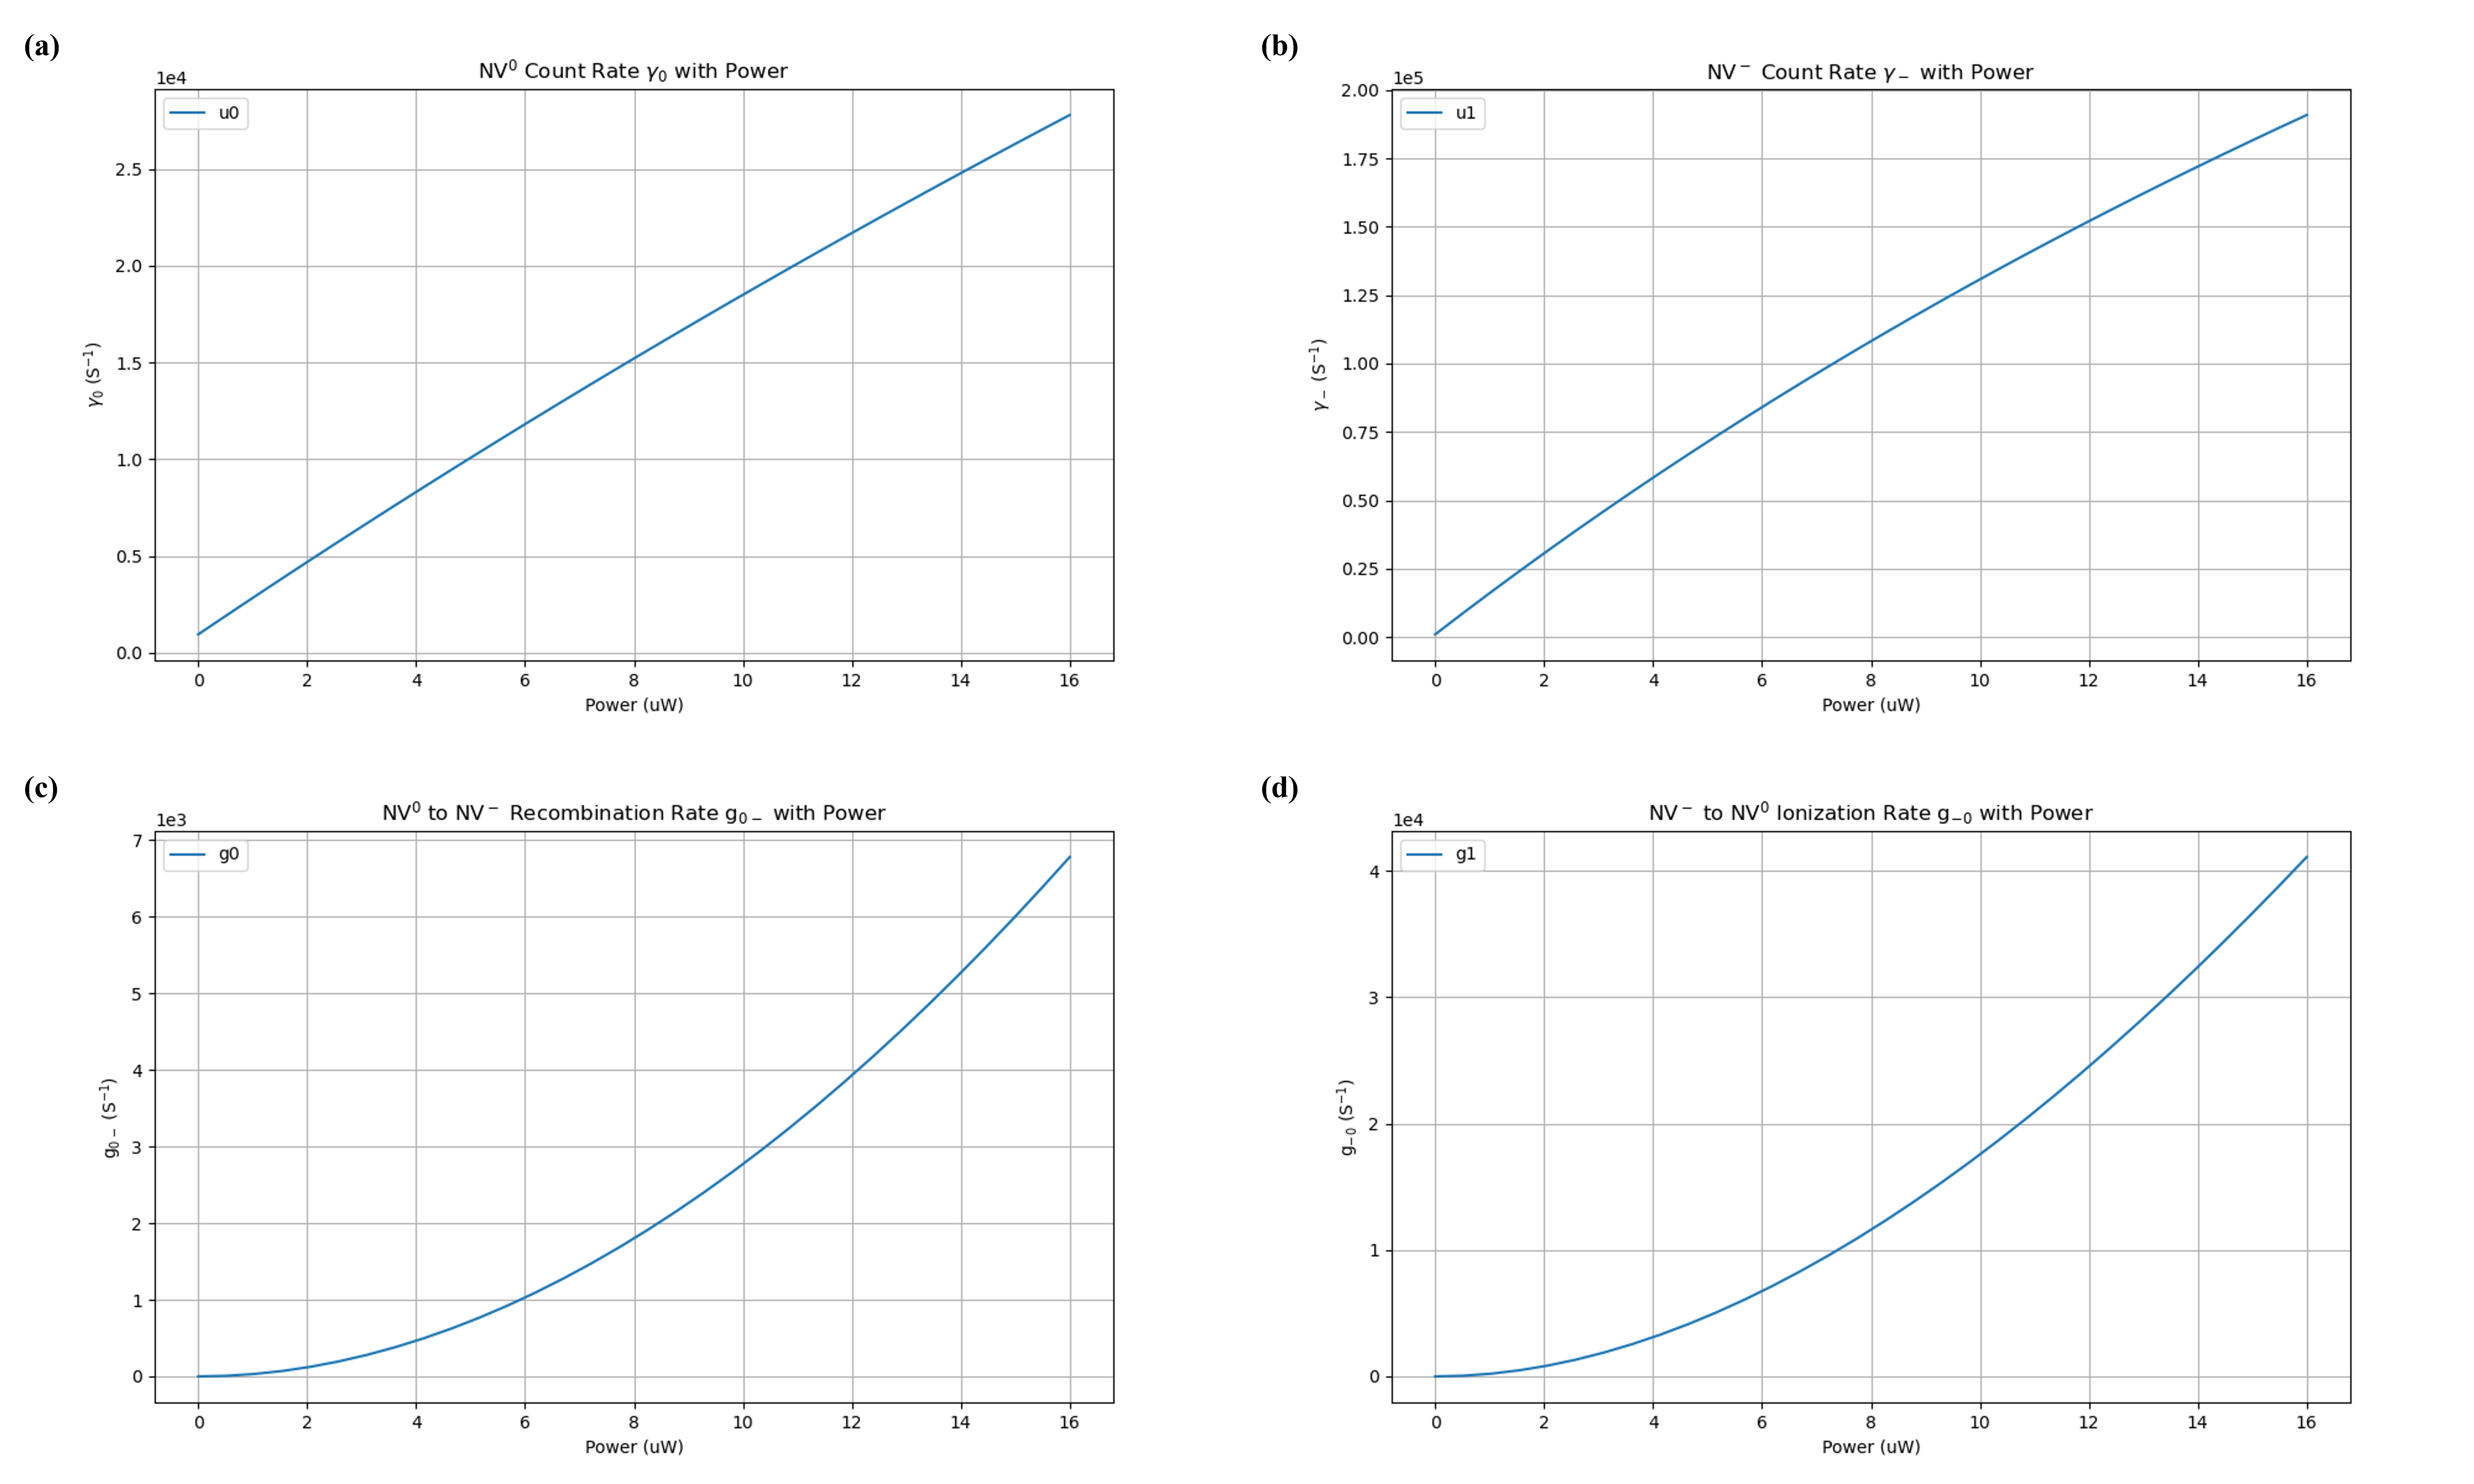
\includegraphics[width=1.0\textwidth]{figures/Chapter 5/P_variation_parameters.png}
  \caption[$\gamma_0$、$\gamma_-$、$g_{0-}$、$g_{-0}$随读出功率的变化]{$\gamma_0$、$\gamma_-$、$g_{0-}$、$g_{-0}$随读出功率的变化。}
  \label{fig: P_variation_parameters}
\end{figure}
可以看到,在同等读出光强的情况下,NV$^-$($\sim 10^5$)的计数率$\gamma_-$相比于NV$^0$($\sim 10^4$)的计数率$\gamma_0$的计数率提高了一个量级,所以在光子数概率分布曲线中可以明显的分辨出两个不同的峰值。当然这是在理想情况下的结果,实际上的测试效果得到的计数率和光路的激发效率、收集效率、单点色心的质量相关,对于同一个单点NV Center而言,这个理论的数值仿真结果得到的数量级关系可以在实验中起到一定的参考价值。在较低光强($0 \sim 16\ \mu W$)的情况下,如图 \ref{fig: P_variation_parameters}(a)和(b),NV$^0$和NV$^-$的计数率$\gamma_0$和$\gamma_-$和光强功率之间近似使正相关的关系;而当光强继续增大的时候($0 \sim 1000\ \mu W$),两者会趋于饱和,这和实际实验中测得的饱和光强曲线结果也是吻合的,如图 \ref{fig: P_saturation}所示,可以看到计数率逐渐饱和的现象,变化趋势类似于对数函数。
\begin{figure}
  \centering
  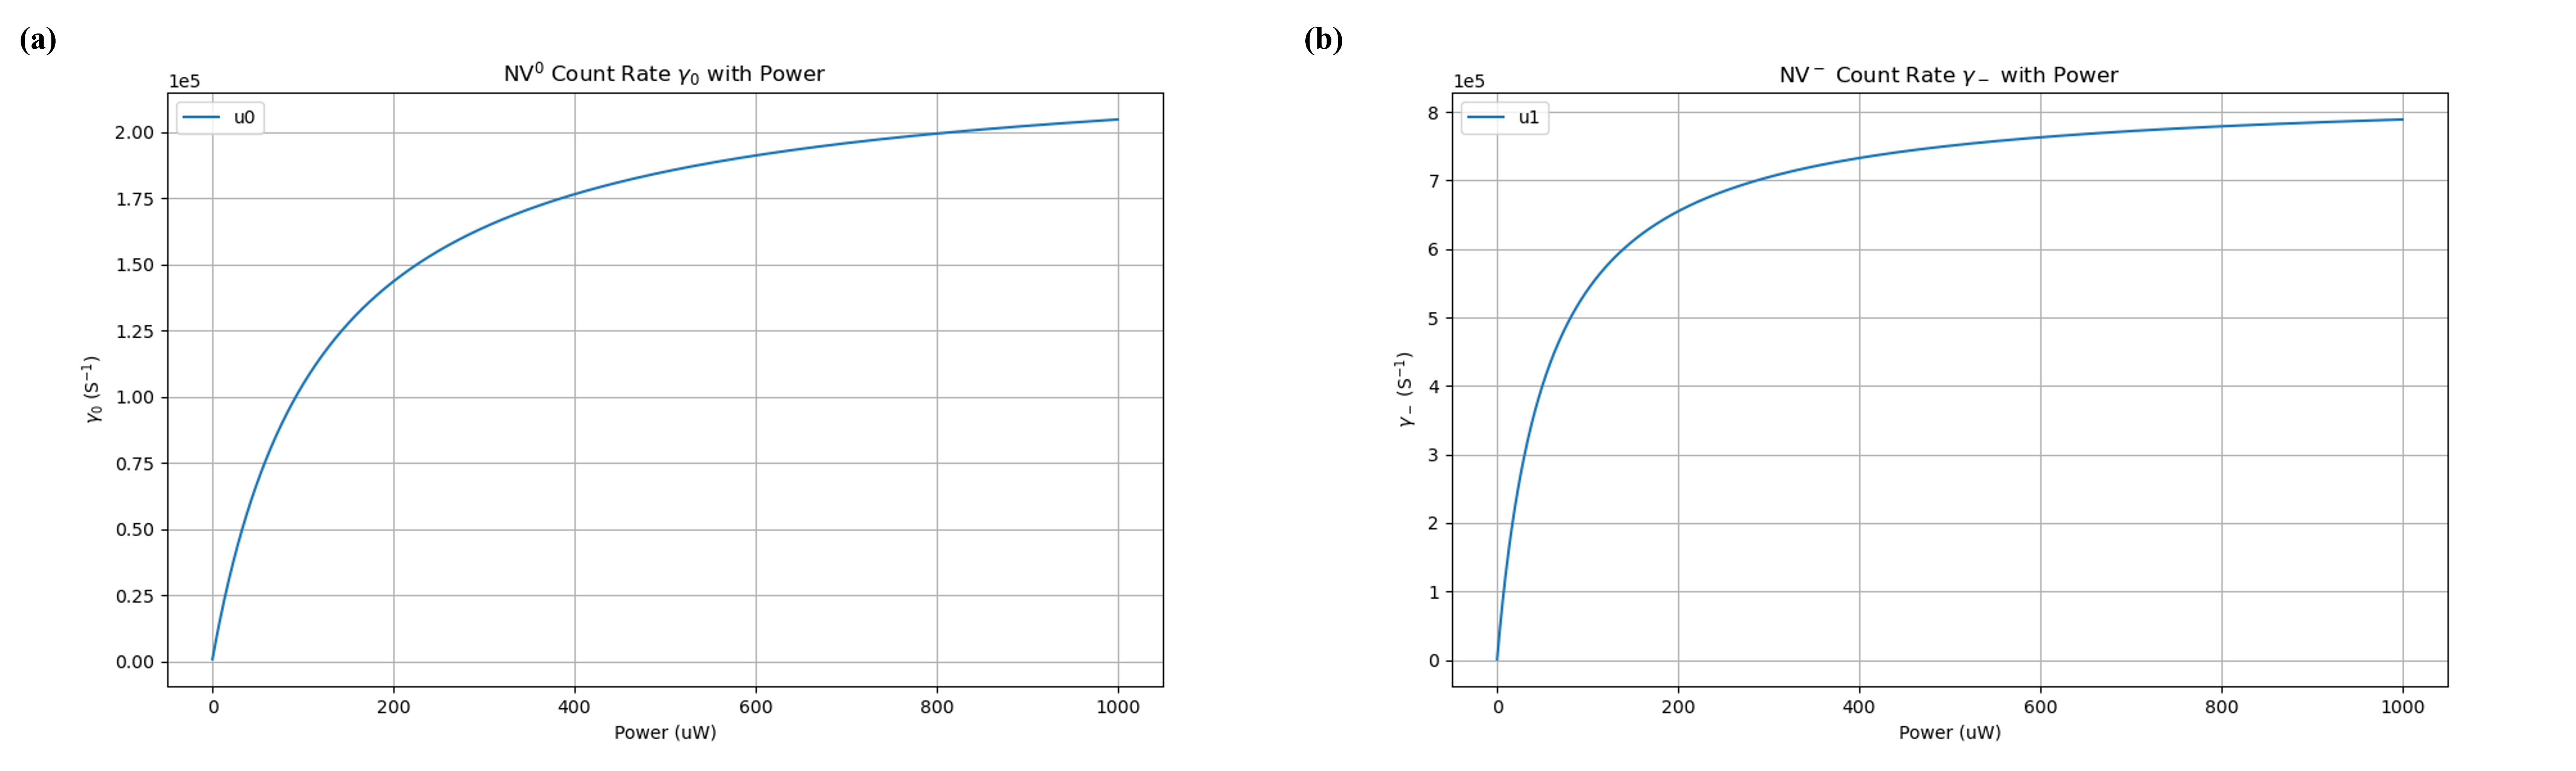
\includegraphics[width=1.0\textwidth]{figures/Chapter 5/P_saturation.png}
  \caption[$\gamma_0$和$\gamma_-$在光强较高的情况下随光强变化的曲线]{$\gamma_0$和$\gamma_-$在光强较高的情况下随光强变化的曲线。}
  \label{fig: P_saturation}
\end{figure}
见图 \ref{fig: P_variation_parameters}(c)和(d),同等光强下,NV$^-$ $\rightarrow$ NV$^0$的转换率$g_{-0}$($\sim 10^4$)相比于NV$^0$ $\rightarrow$ NV$^-$的转换率$g_{0-}$($\sim 10^3$),而且$g_{0-}/g_{-0}$之间的比值随着功率而升高,如图 \ref{fig: g0_g1_ratio}(a)所示。
\begin{figure}
  \centering
  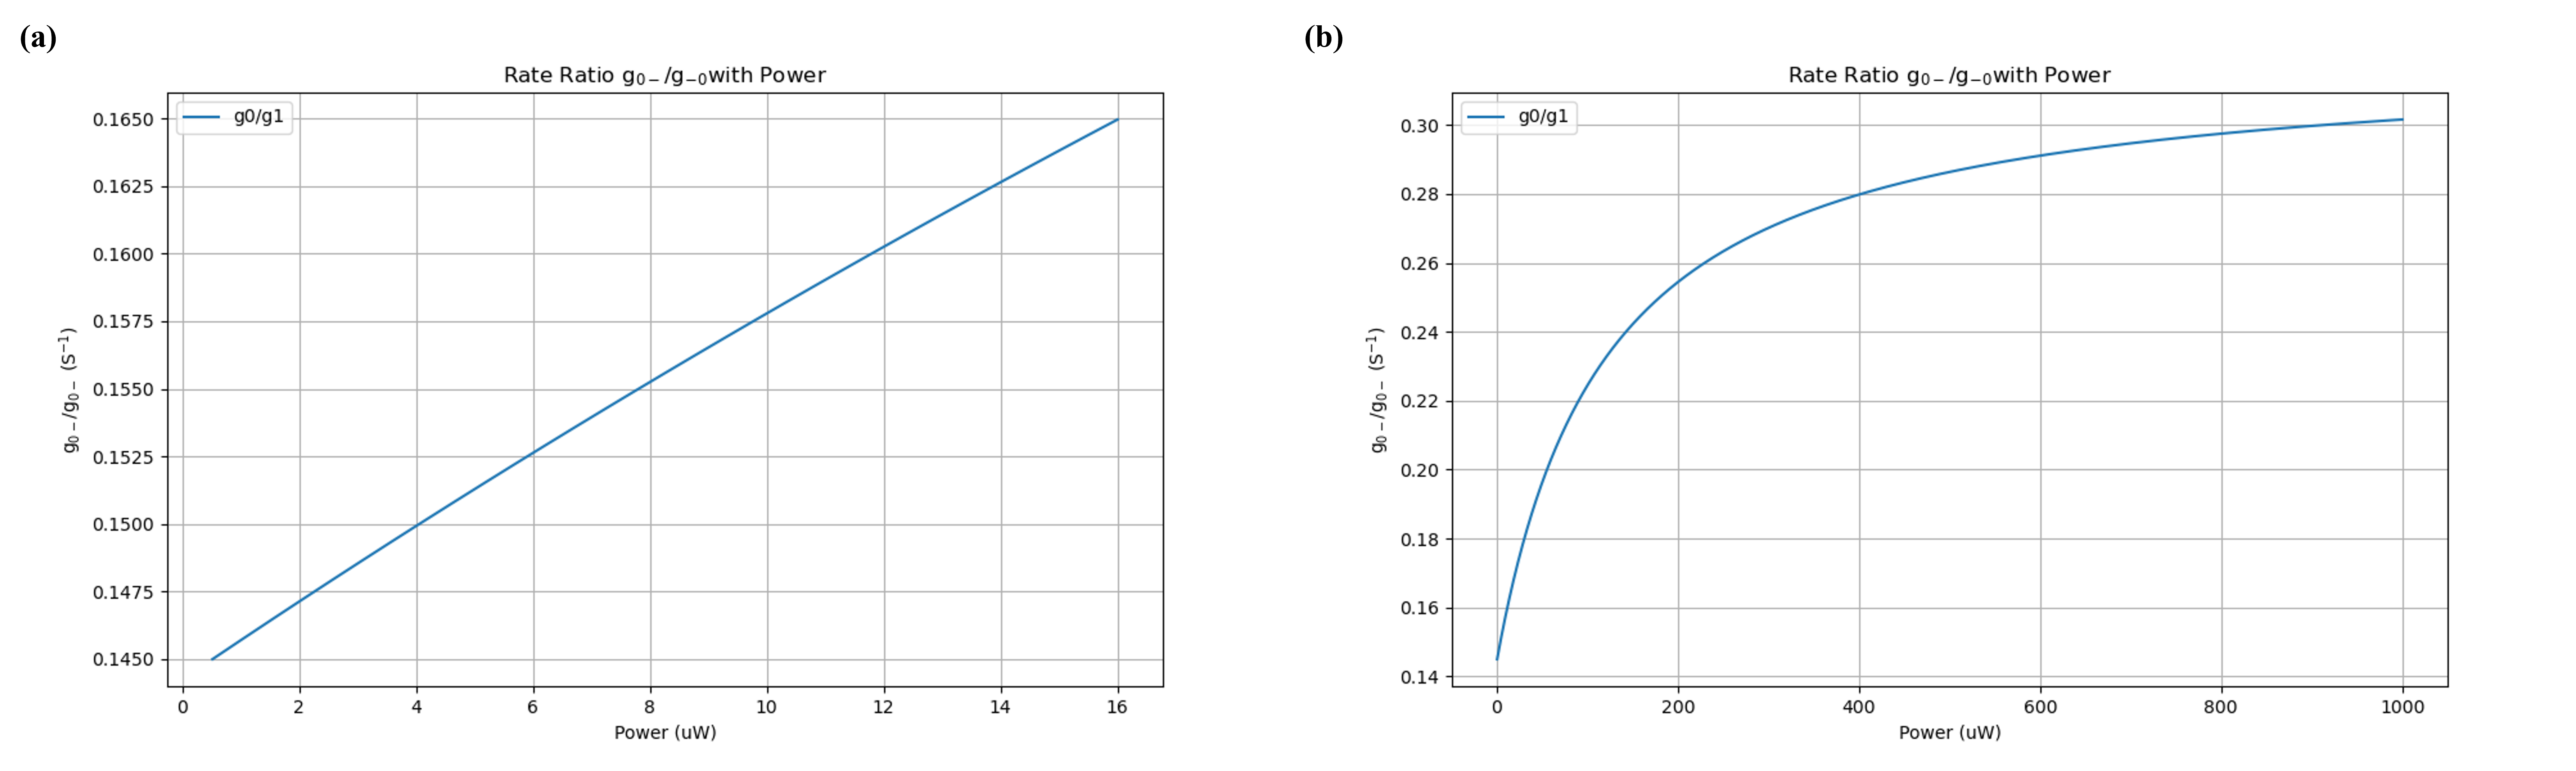
\includegraphics[width=1.0\textwidth]{figures/Chapter 5/g0_g1_ratio.png}
  \caption[$g_{0-}$和$g_{-0}$的比值在不同光强范围相对于光强的变化曲线]{$g_{0-}$和$g_{-0}$的比值在不同光强范围相对于光强的变化曲线,(a)光强范围为$0 \sim 16\ \mu W$,(b)光强范围为$0 \sim 1000\ \mu W$。}
  \label{fig: g0_g1_ratio}
\end{figure}
在CW测量下,要维持NV$^-$和NV$^0$之间的动态平衡,也就是:
\begin{equation}
  \eta(NV^-) \cdot g_{-0} = \eta(NV^0) \cdot g_{0-}
\end{equation}
\begin{equation}
  \frac{g_{0-}}{g_{-0}} = \frac{\eta(NV^-)}{\eta(NV^0)}
\end{equation}
其中$\eta$为NV不同电荷态的占比,可以看到随着读出的594 nm橙光激光功率的增加,NV$^-$的比例越高,也符合实验的结果。不过值得注意的是,这种简单的分析方法仅可用于定性分析观察探究变化趋势,用于定量分析会有一些不严谨的地方。比如在这种条件下,读出光强较高的时候,如图 \ref{fig: g0_g1_ratio}(b)所示,在$0 \sim 1000\ \mu W$的光强范围尺度下,$g_{0-}$和$g_{-0}$的比值区域收敛。实际上NV$^-$和NV$^0$之间的分布情况还取决于NV Center本身的性质和环境条件的影响,比如表面负电性的因素。一个常见的情况就是在三酸洗(浓硫酸、浓硝酸和高氯酸)之后,金刚石的表面会形成氧终端面(O-terminated surface),使得金刚石的电子亲合能提高,NV$^-$的占比更高。

我们通过数值仿真探究了不同光强下的概率分布曲线,如图 \ref{fig: P_var_dist}所示
\begin{figure}
  \centering
  \includegraphics[width=1.0\textwidth]{figures/Chapter 5/P_var_dist.png}
  \caption[不同读出功率下NV$^0$和NV$^-$的概率分布曲线]{不同读出功率下NV$^0$和NV$^-$的概率分布曲线,从(a)到(h)光强逐渐升高。}
  \label{fig: P_var_dist}
\end{figure}
根据不同的读出功率$P_{594}$,其过程状态参数如 \ref{tab: P_variation_parameters}所示:

\begin{table}[ht]
  \centering
  \caption{不同读出功率下$t_r$、$\gamma_0$、$\gamma_-$、$g_{0-}$、$g_{-0}$的计算结果和拟合参数设置}
  \label{tab: P_variation_parameters}
  \begin{tabularx}{\textwidth}{CCCCCC}
    \toprule
    $P_{594}\ (\mu W)$ & $t_r\ (ms)$ & $\gamma_0\ (s^{-1})$ & $\gamma_-\ (s^{-1})$ & $g_{0-}\ (s^{-1})$ & $g_{-0}\ (s^{-1})$ \\
    \midrule
    0.5 & 14 & 1896.56 & 8571.43 & 7.47 & 51.52 \\
    1 & 8.5 & 2835.29 & 16054.29 & 29.75 & 204.22 \\
    2 & 2.5 & 4689.67 & 30619.14 & 118.03 & 802.29 \\
    3 & 1.5 & 6513.90 & 44672.95 & 263.41 & 1773.47 \\
    5 & 1.0 & 10074.80 & 71351.36 & 720.00 & 4759.32 \\
    7 & 0.3 & 13523.54 & 96280.36 & 1388.98 & 9022.43 \\
    9 & 0.3 & 16865.35 & 119626.57 & 2260.47 & 14441.14 \\
    11 & 0.2 & 20105.11 & 141536.09 & 3325.19 & 20908.80 \\
    \bottomrule
  \end{tabularx}
\end{table}
从(a)到(h)光强逐渐升高,而读出时间是根据横轴的数据来进行选择和调整的。当光强较小的时候,需要更大的$t_r$来使得其累计足够的光子数便于获得更多的数据点进行拟合绘图,而当光强较大的时候,由于光子数较多,可以选择较小的$t_r$来获得更高的分辨率。在图 \ref{fig: P_tR_dist}所示,可以看到在$P_{594}=11.0\ \mu W$的条件下,$t_r = 0.05,\ 0.2,\ 2.0,\ 10.0\ ms$的概率分布曲线,可以看到过小的$t_r$得到的数据量较小,曲线的形状比较粗糙;而较大的$t_r$会使得两个峰之间的分辨率降低,最后形成一个峰,不具有区分性。
\begin{figure}
  \centering
  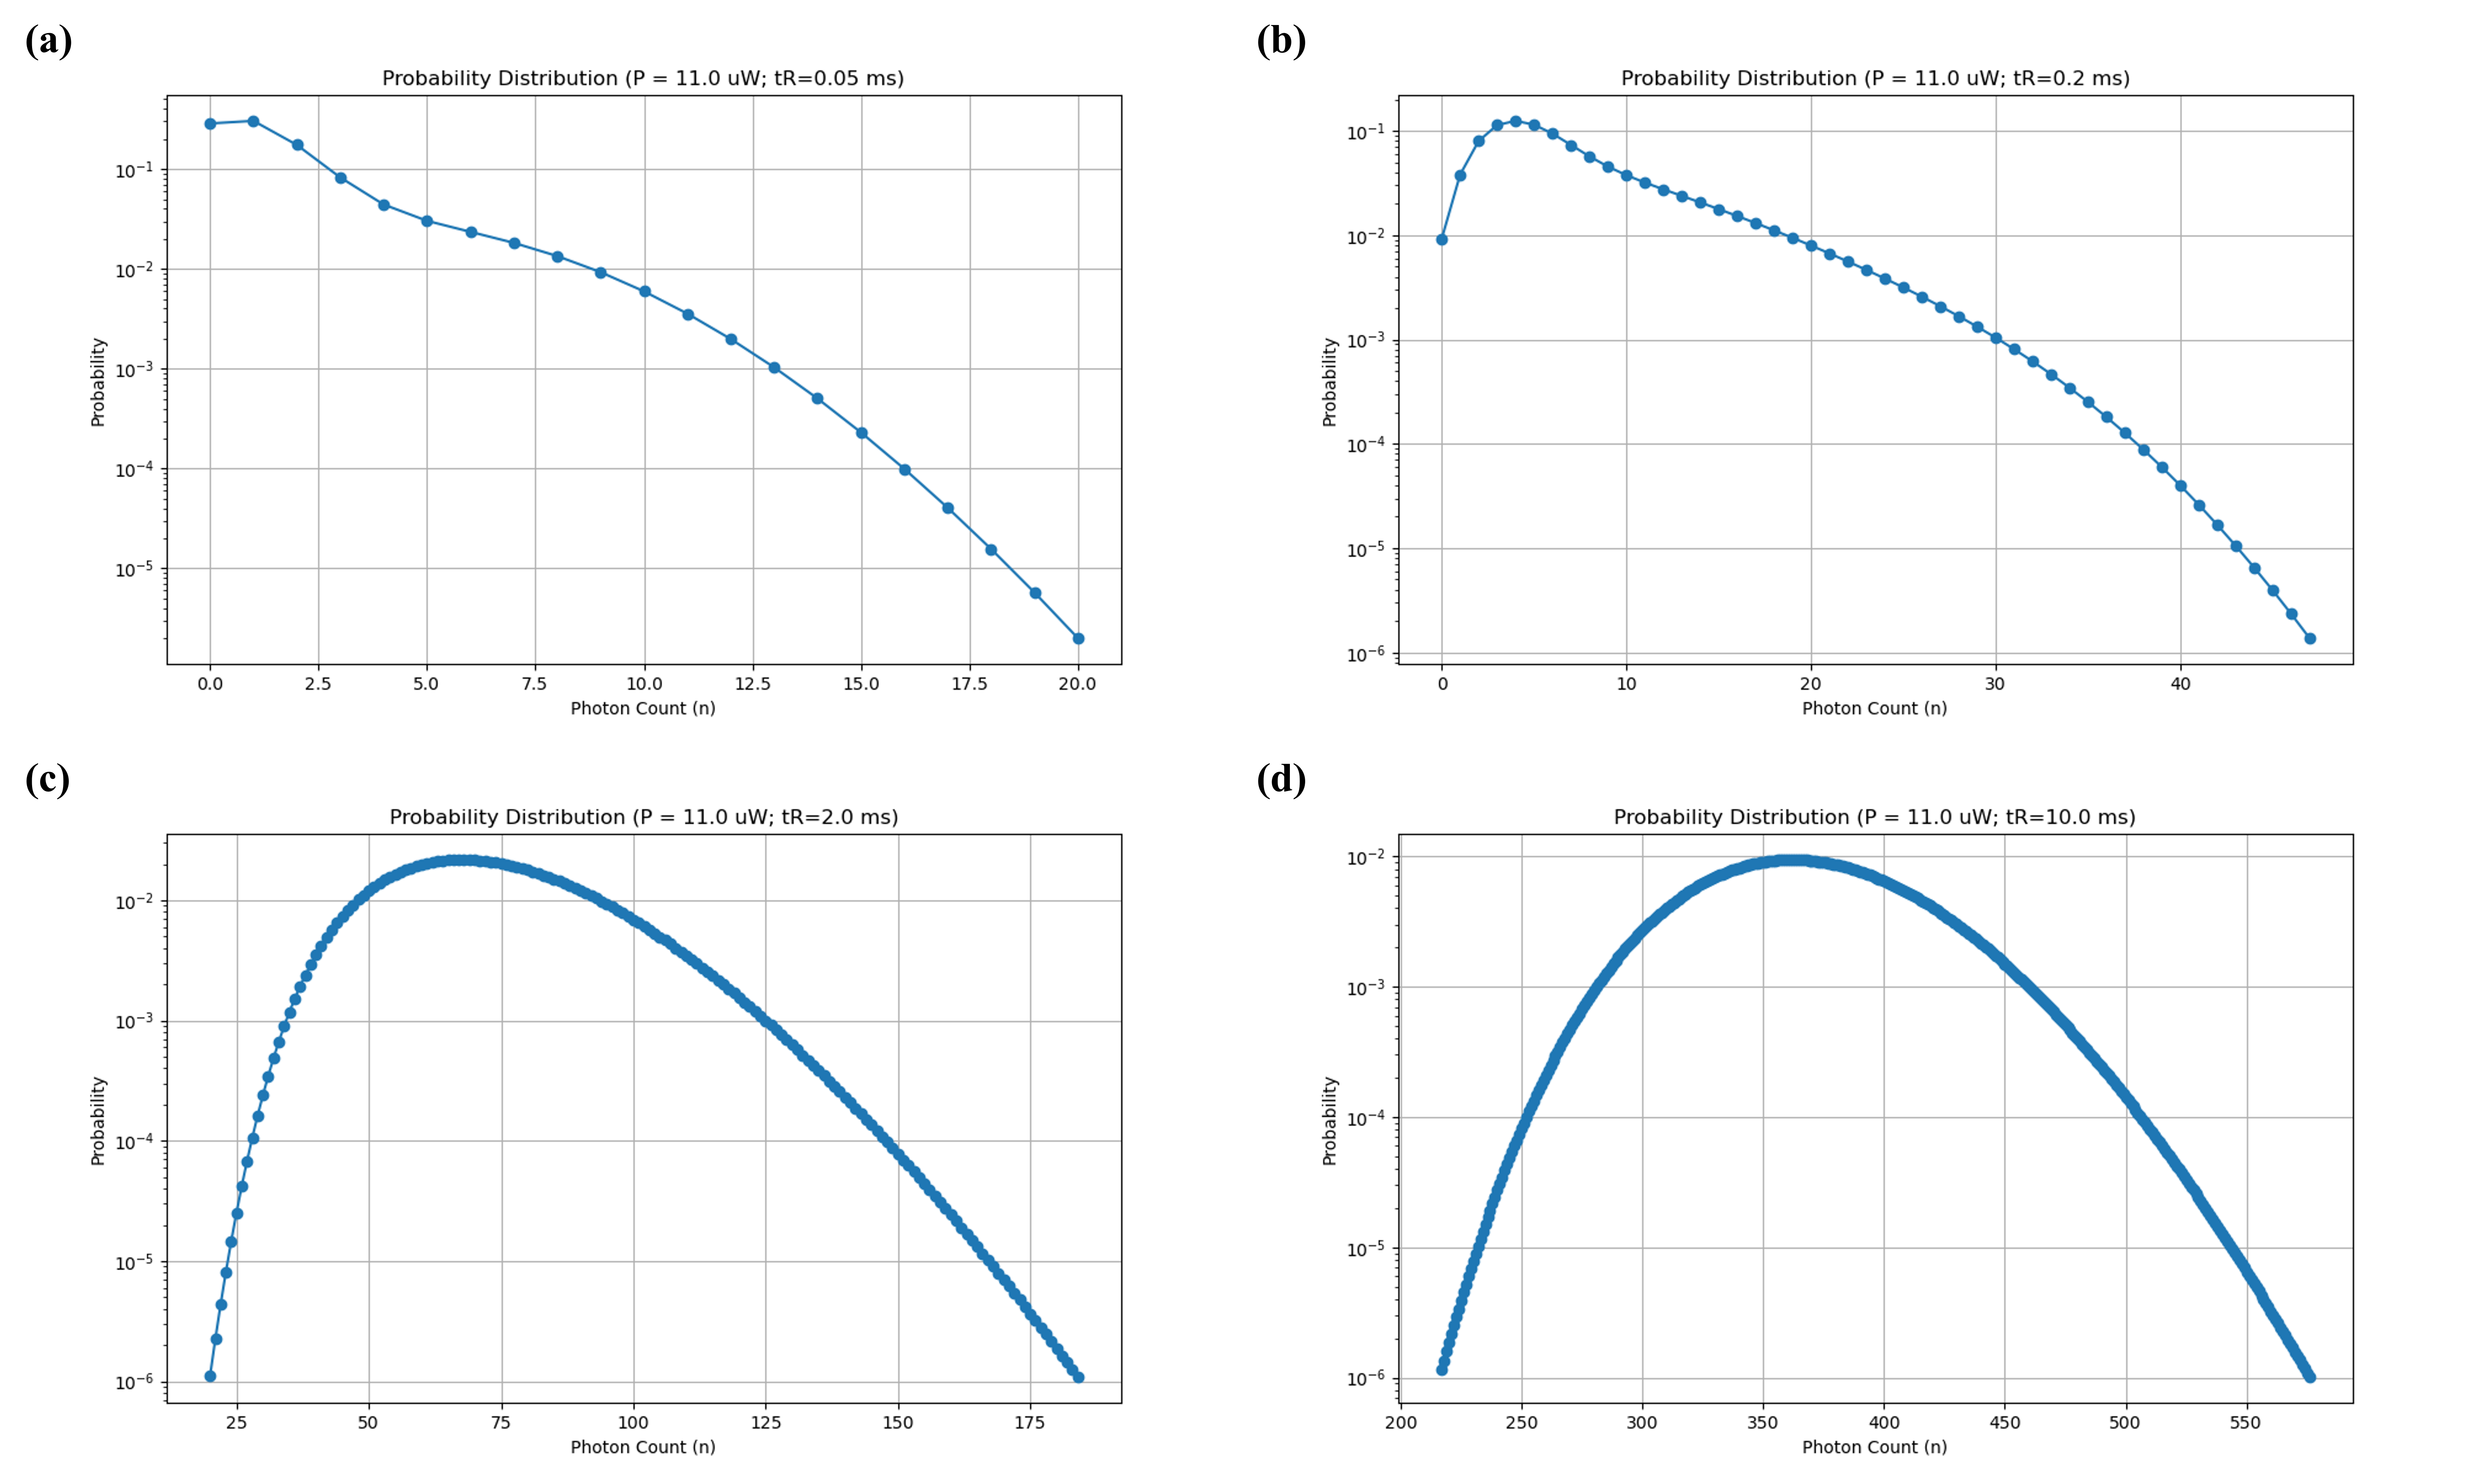
\includegraphics[width=1.0\textwidth]{figures/Chapter 5/P_tR_dist.png}
  \caption[$P_{594}=11.0\ \mu W$的情况下,概率分布曲线随$t_r$的变化]{$P_{594}=11.0\ \mu W$的情况下,概率分布曲线随$t_r$的变化。}
  \label{fig: P_tR_dist}
\end{figure}
横轴的范围选择也可以作为$t_r$选择的一个依据,一般是遵循三种方法:第一种是概率高于一个设置的阈值,一般设置为10$^{-7}$附近的范围及其更高的部分;第二种方式就是在功率$P_{594}$取不同的值的时候,横轴的数值大致相近;最后一种方式是看整个曲线形状,在必要的时候需要调整横轴的范围,使得曲线的形状更加完整,便于观察和分析。通过图中的对比可以看到,在读出功率$P_{594}$较小的时候,两个峰值之间会更易于区分,对比度较高,更好的区分出NV$^0$和NV$^-$的电荷态分布情况;而当光强较大的时候,两个峰值之间的区分度会降低,这是因为两个峰值之间的距离会变小,而且两个峰值的高度差异也会变小,这样就会使得两个峰值之间的区分度降低,这也是实验中在较高光强下,两个峰值之间的区分度较低的原因。

读出激光的功率$P_{594}$不宜选取过大的值,如图 \ref{fig: P_var_dist_high}所示
\begin{figure}
  \centering
  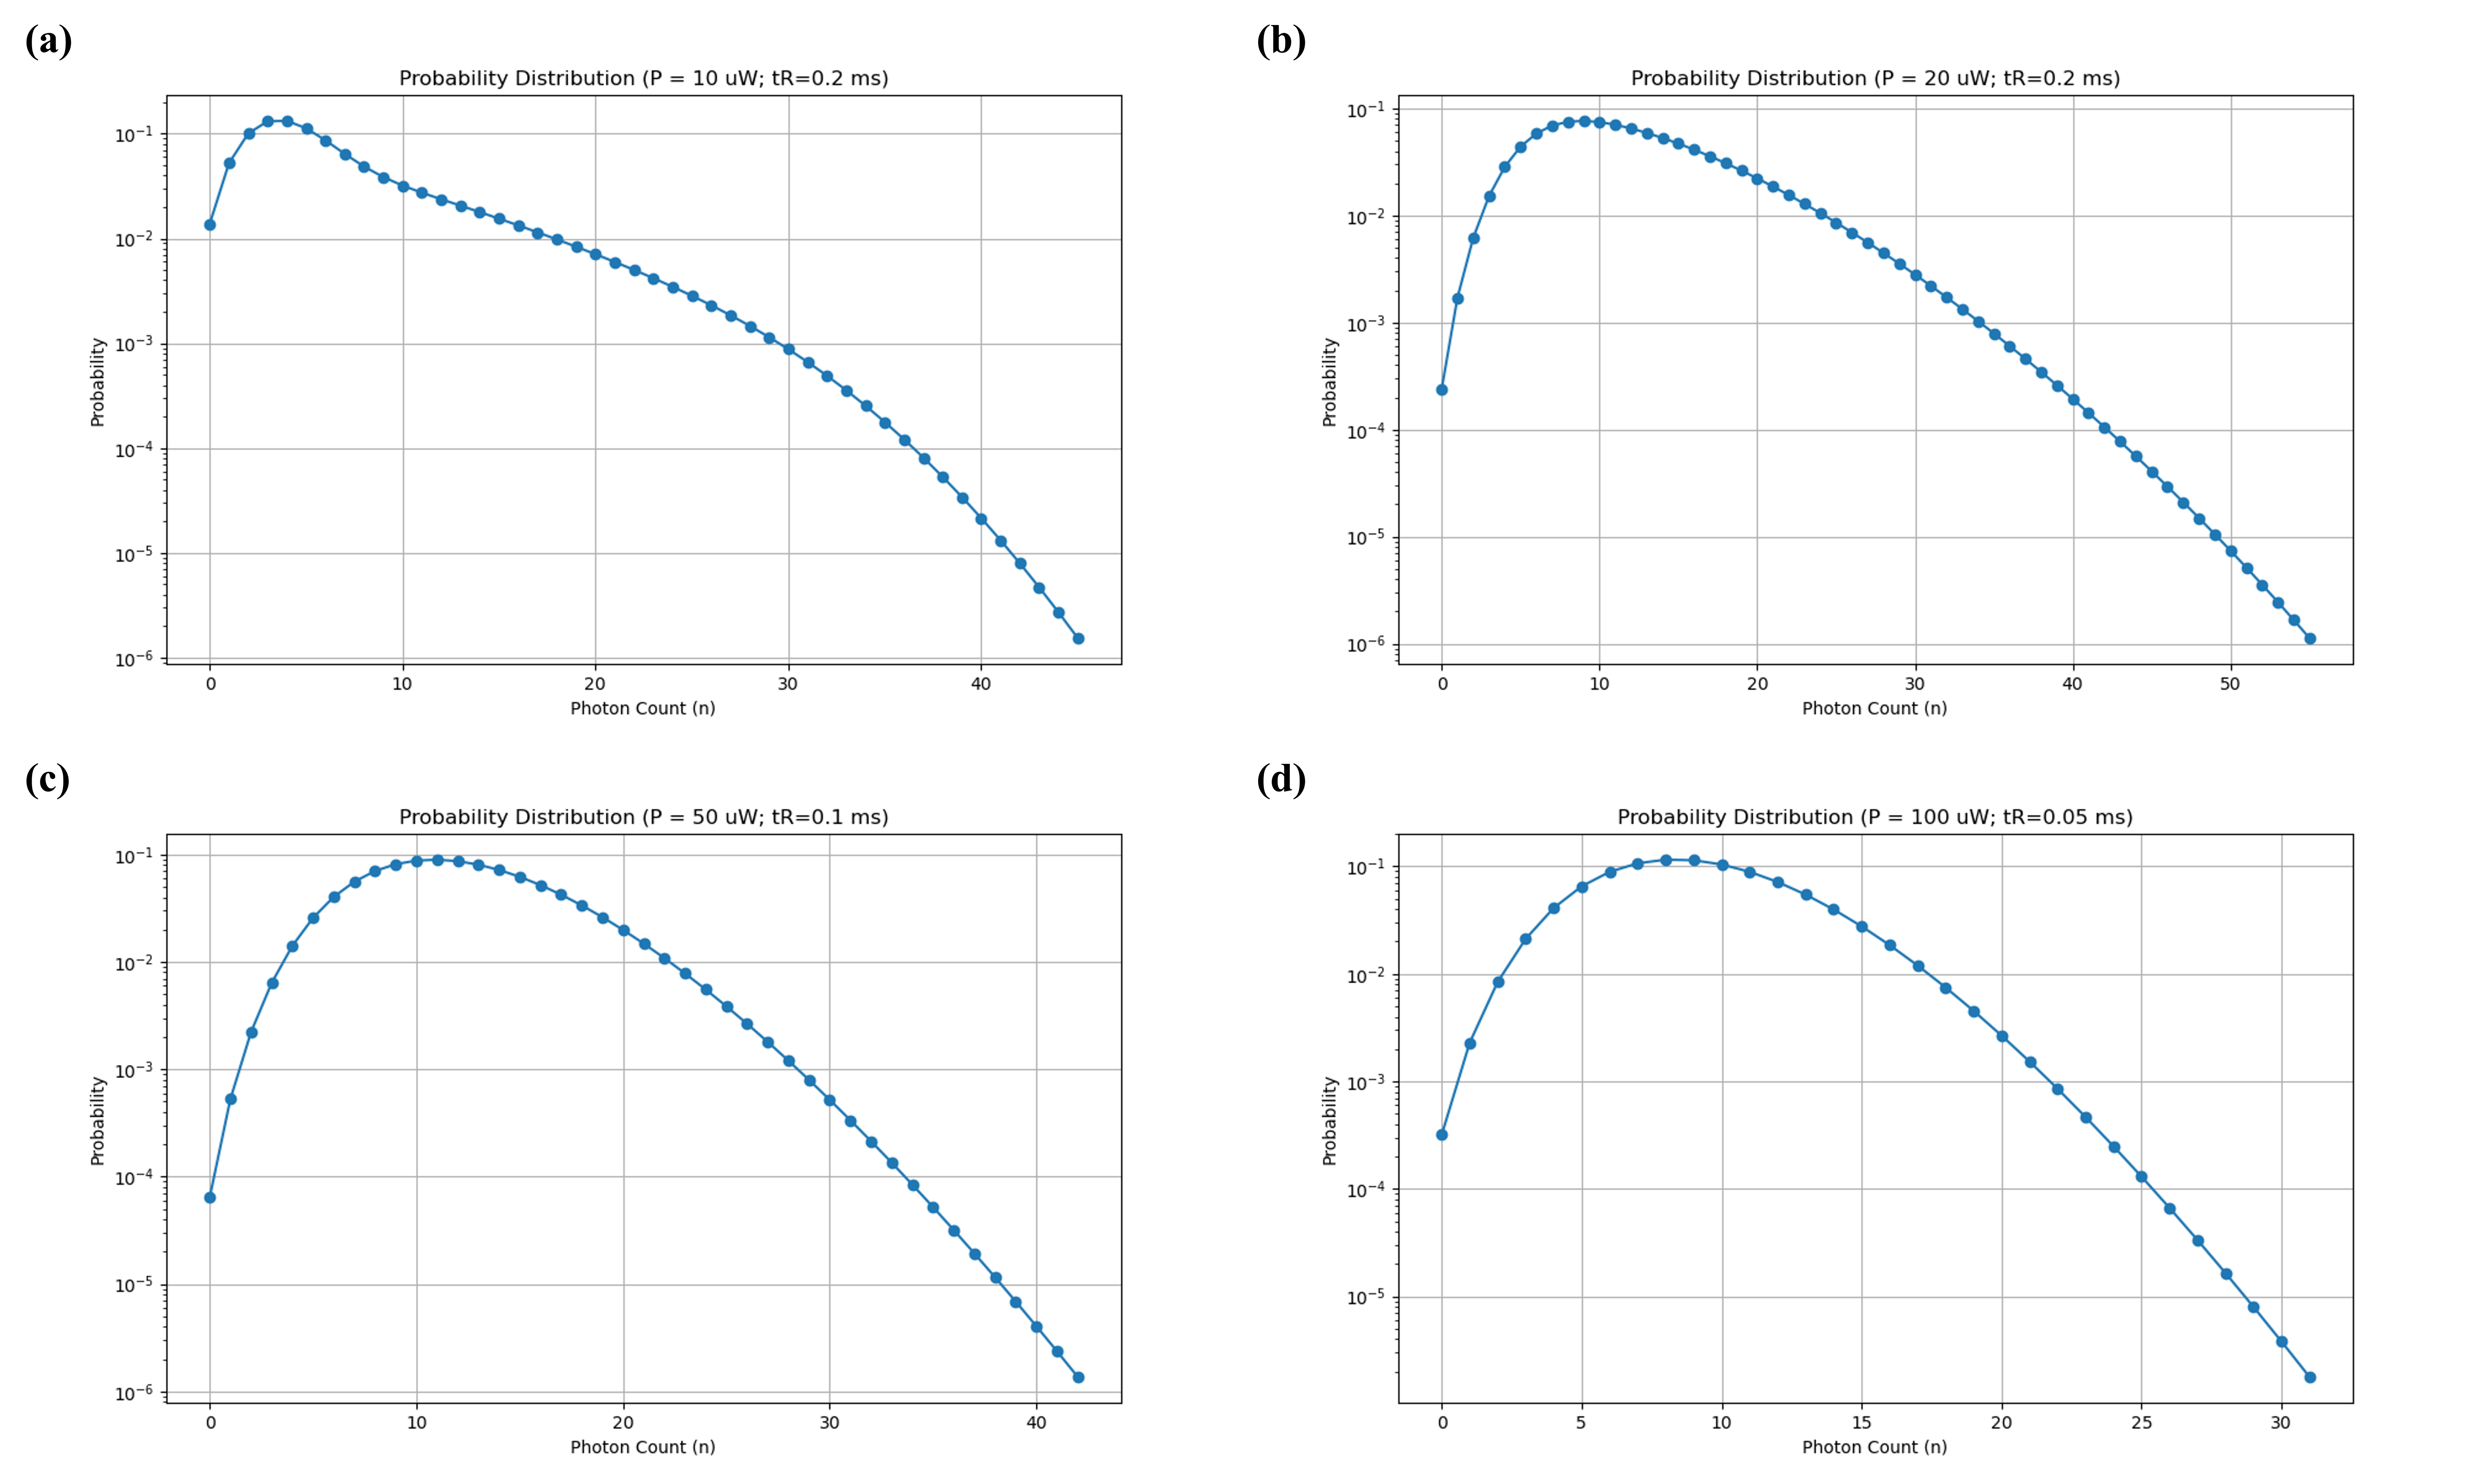
\includegraphics[width=1.0\textwidth]{figures/Chapter 5/P_var_dist_high.png}
  \caption[$P_{594}$较大的情况下,概率分布曲线的变化]{$P_{594}$较大的情况下,概率分布曲线的变化}
  \label{fig: P_var_dist_high}
\end{figure}
当功率较高的时候,只剩下一个峰值,但如果降低$t_r$,数据点的密度就会降低,曲线近乎成为一条直线,无法得到Possion Distribution的特征,这样就无法得到NV$^0$和NV$^-$的电荷态分布情况。降低$P_{594}$读出功率再进行拟合,可以大致看到两个峰的轮廓,如图 \ref{fig: P_var_dist_high}(a)所示。当$P_{594}$读出功率过大的时候,接近或者超过NV$^0$和NV$^-$的饱和光强$P_{Sat,0}$和$P_{Sat,-}$,所以荧光效应接近饱和,难以通过计数率的差别分辨NV$^0$和NV$^-$,从而使得分布数据失效,无法拟合出有效参数。当然,由于环境的震动和杂散光子的影响,以及APD本身的暗计数等因素,光强过低的话会导致得到的数据信噪比较低。因此在实际实验中,需要根据实际情况选择合适且较低的读出激光功率$P_{594}$和读出时间$t_r$,同时延长测量和数据收集的时间,以从而得到最佳的实验效果。

\subsection{不同读出转化率和计数率对概率分布的影响}

在上面的过程中,我们主要是通过改变读出的激光功率$P_{594}$和读出时间$t_r$来探究NV$^0$和NV$^-$的电荷态分布情况,接下来我们将通过改变NV$^0$和NV$^-$的计数率$\gamma_0$和$\gamma_-$,以及NV$^0$到NV$^-$的结合速率$g_{0-}$和NV$^-$到NV$^0$的电离速率$g_{-0}$来探究概率分布的变化情况。

\subsubsection{$t_r$,$\gamma_0$,$\gamma_-$固定的情况下,改变$g_{0-}$和$g_{-0}$}
在这个过程中,我们将固定读出时间$t_r = 15.0\ ms$,NV$^0$的计数率$\gamma_0 = 1803\ s^{-1}$,NV$^-$的计数率$\gamma_- = 8090\ s^{-1}$,改变NV$^0$ $\rightarrow$ NV$^-$的转换率$g_{0-}$和NV$^-$ $\rightarrow$ NV$^0$的转换率$g_{-0}$,得到图 \ref{fig: g_variation}中的概率分布曲线。
\begin{figure}
  \centering
  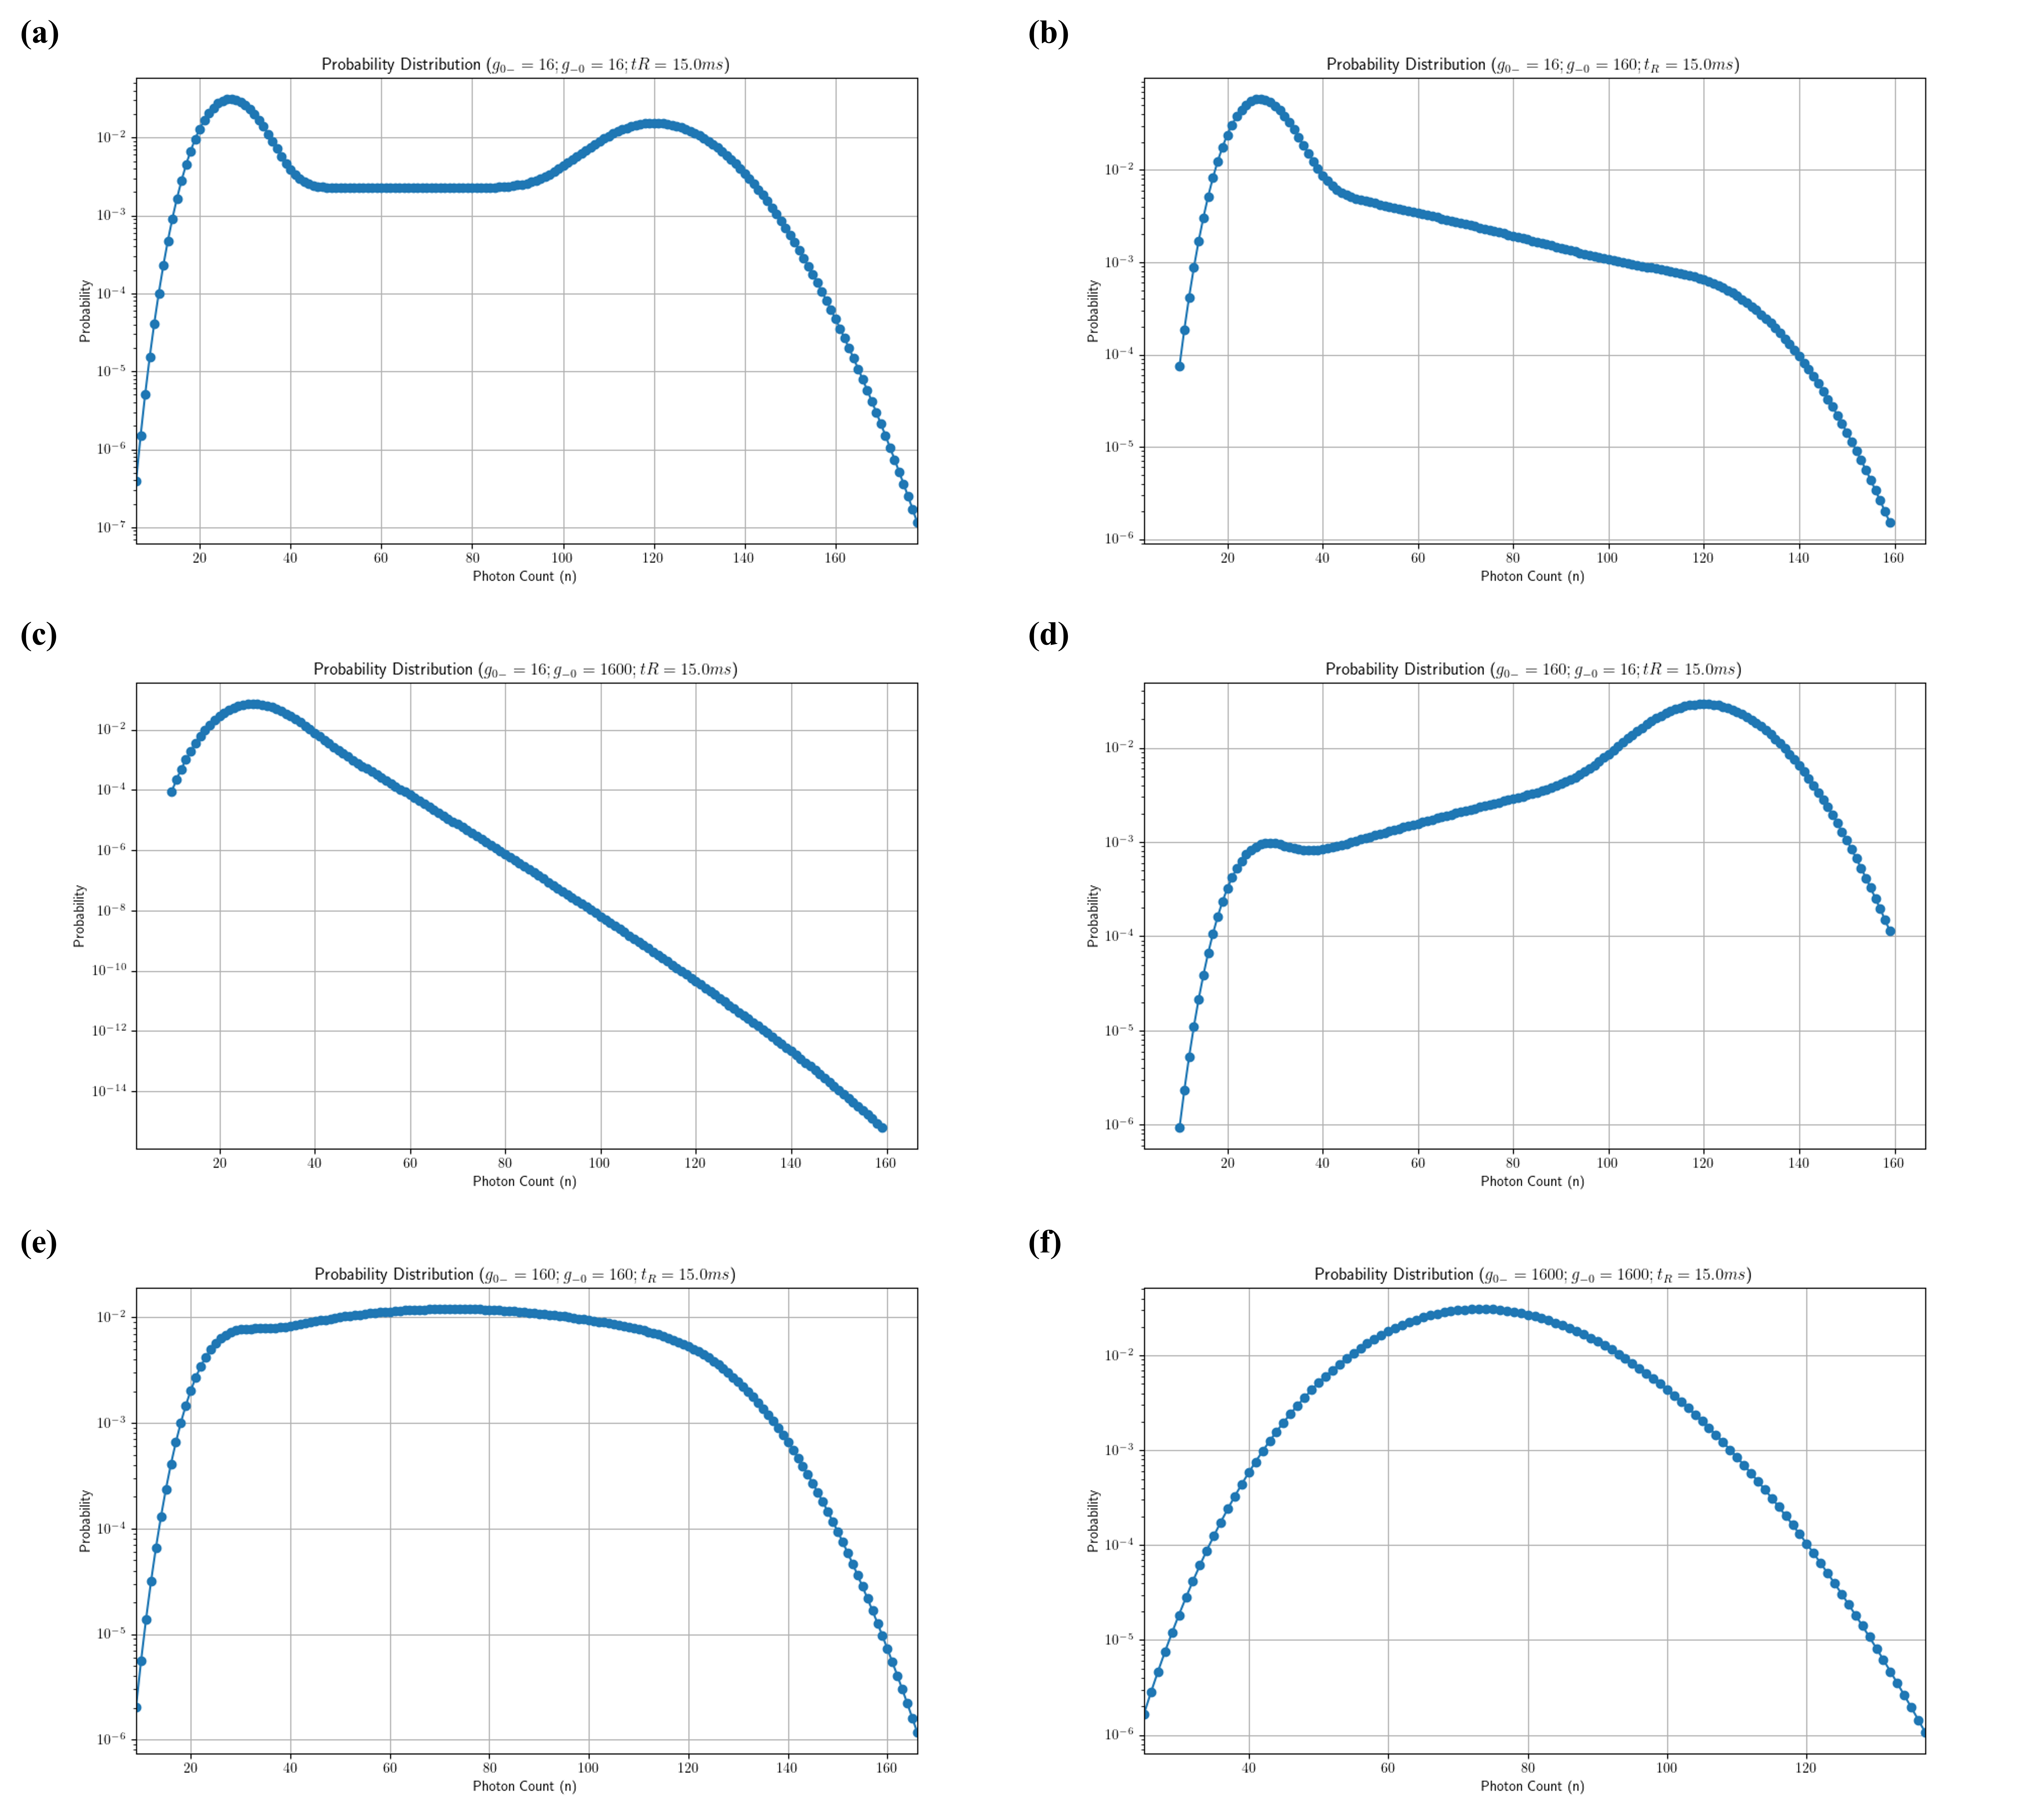
\includegraphics[width=1.0\textwidth]{figures/Chapter 5/g_variation.png}
  \caption[$t_r = 15.0\ ms$,$\gamma_0 = 1803\ s^{-1}$,$\gamma_- = 8090\ s^{-1}$的情况下,改变$g_{0-}$和$g_{-0}$($s^{-1}$)得到的概率分布曲线]{$t_r = 15.0\ ms$,$\gamma_0 = 1803\ s^{-1}$,$\gamma_- = 8090\ s^{-1}$的d情况下,改变$g_{0-}$和$g_{-0}$得到的概率分布曲线}
  \label{fig: g_variation}
\end{figure}
可以看到,$g_{0-}$和$g_{-0}$的比值决定了两个峰的相对高度,$g_{0-}>g_{-0}$则表明NV$^0$ $\rightarrow$ NV$^-$转化的速率更高,NV$^-$的占比更多,则曲线右边的峰值较高;反之,$g_{0-}<g_{-0}$则表明NV$^-$ $\rightarrow$ NV$0$转化的速率更高,NV$^0$的占比更多,则曲线左边的峰值较高。当$g_{0-}$或$g_{-0}$的值变大的时候,即从16 $\rightarrow$ 160 $\rightarrow$ 1600的过程中,在$t_r$不变的情况下,两个峰的可分辨性越来越低。当$g_{0-}$或$g_{-0}$特别很大的时候,如图 \ref{fig: g_variation}(b)所示,$g_{0-}\ll g_{-0}$的情况下,可以看到只出现一个峰,可能的原因是基本上NV$^-$全部向NV$^0$的方向转换。当$g_{0-}$和$g_{-0}$两个值都特别很大的时候,如图 \ref{fig: g_variation}(d)所示,由于当$g_{0-}$或$g_{-0}$都和读出功率$P_{594}$呈正相关,所以这种情况下达到了饱和,只能出现一个峰值,和前面分析的结果一致。这个时候即使是改变$t_r$,也无法分辨出两个峰值,如图 \ref{fig: g_large_tR_variation}展示了$g_{0-} = g_{-0} = 1600\ s^{-1}$的情况下,取$t_r = 0.5,\ 1.5,\ 5.0,\ 15.0,\ 50.0,\ 150.0\ ms$得到的概率分布曲线,可以看到所有的情况下都只会出现一个峰值。
\begin{figure}
  \centering
  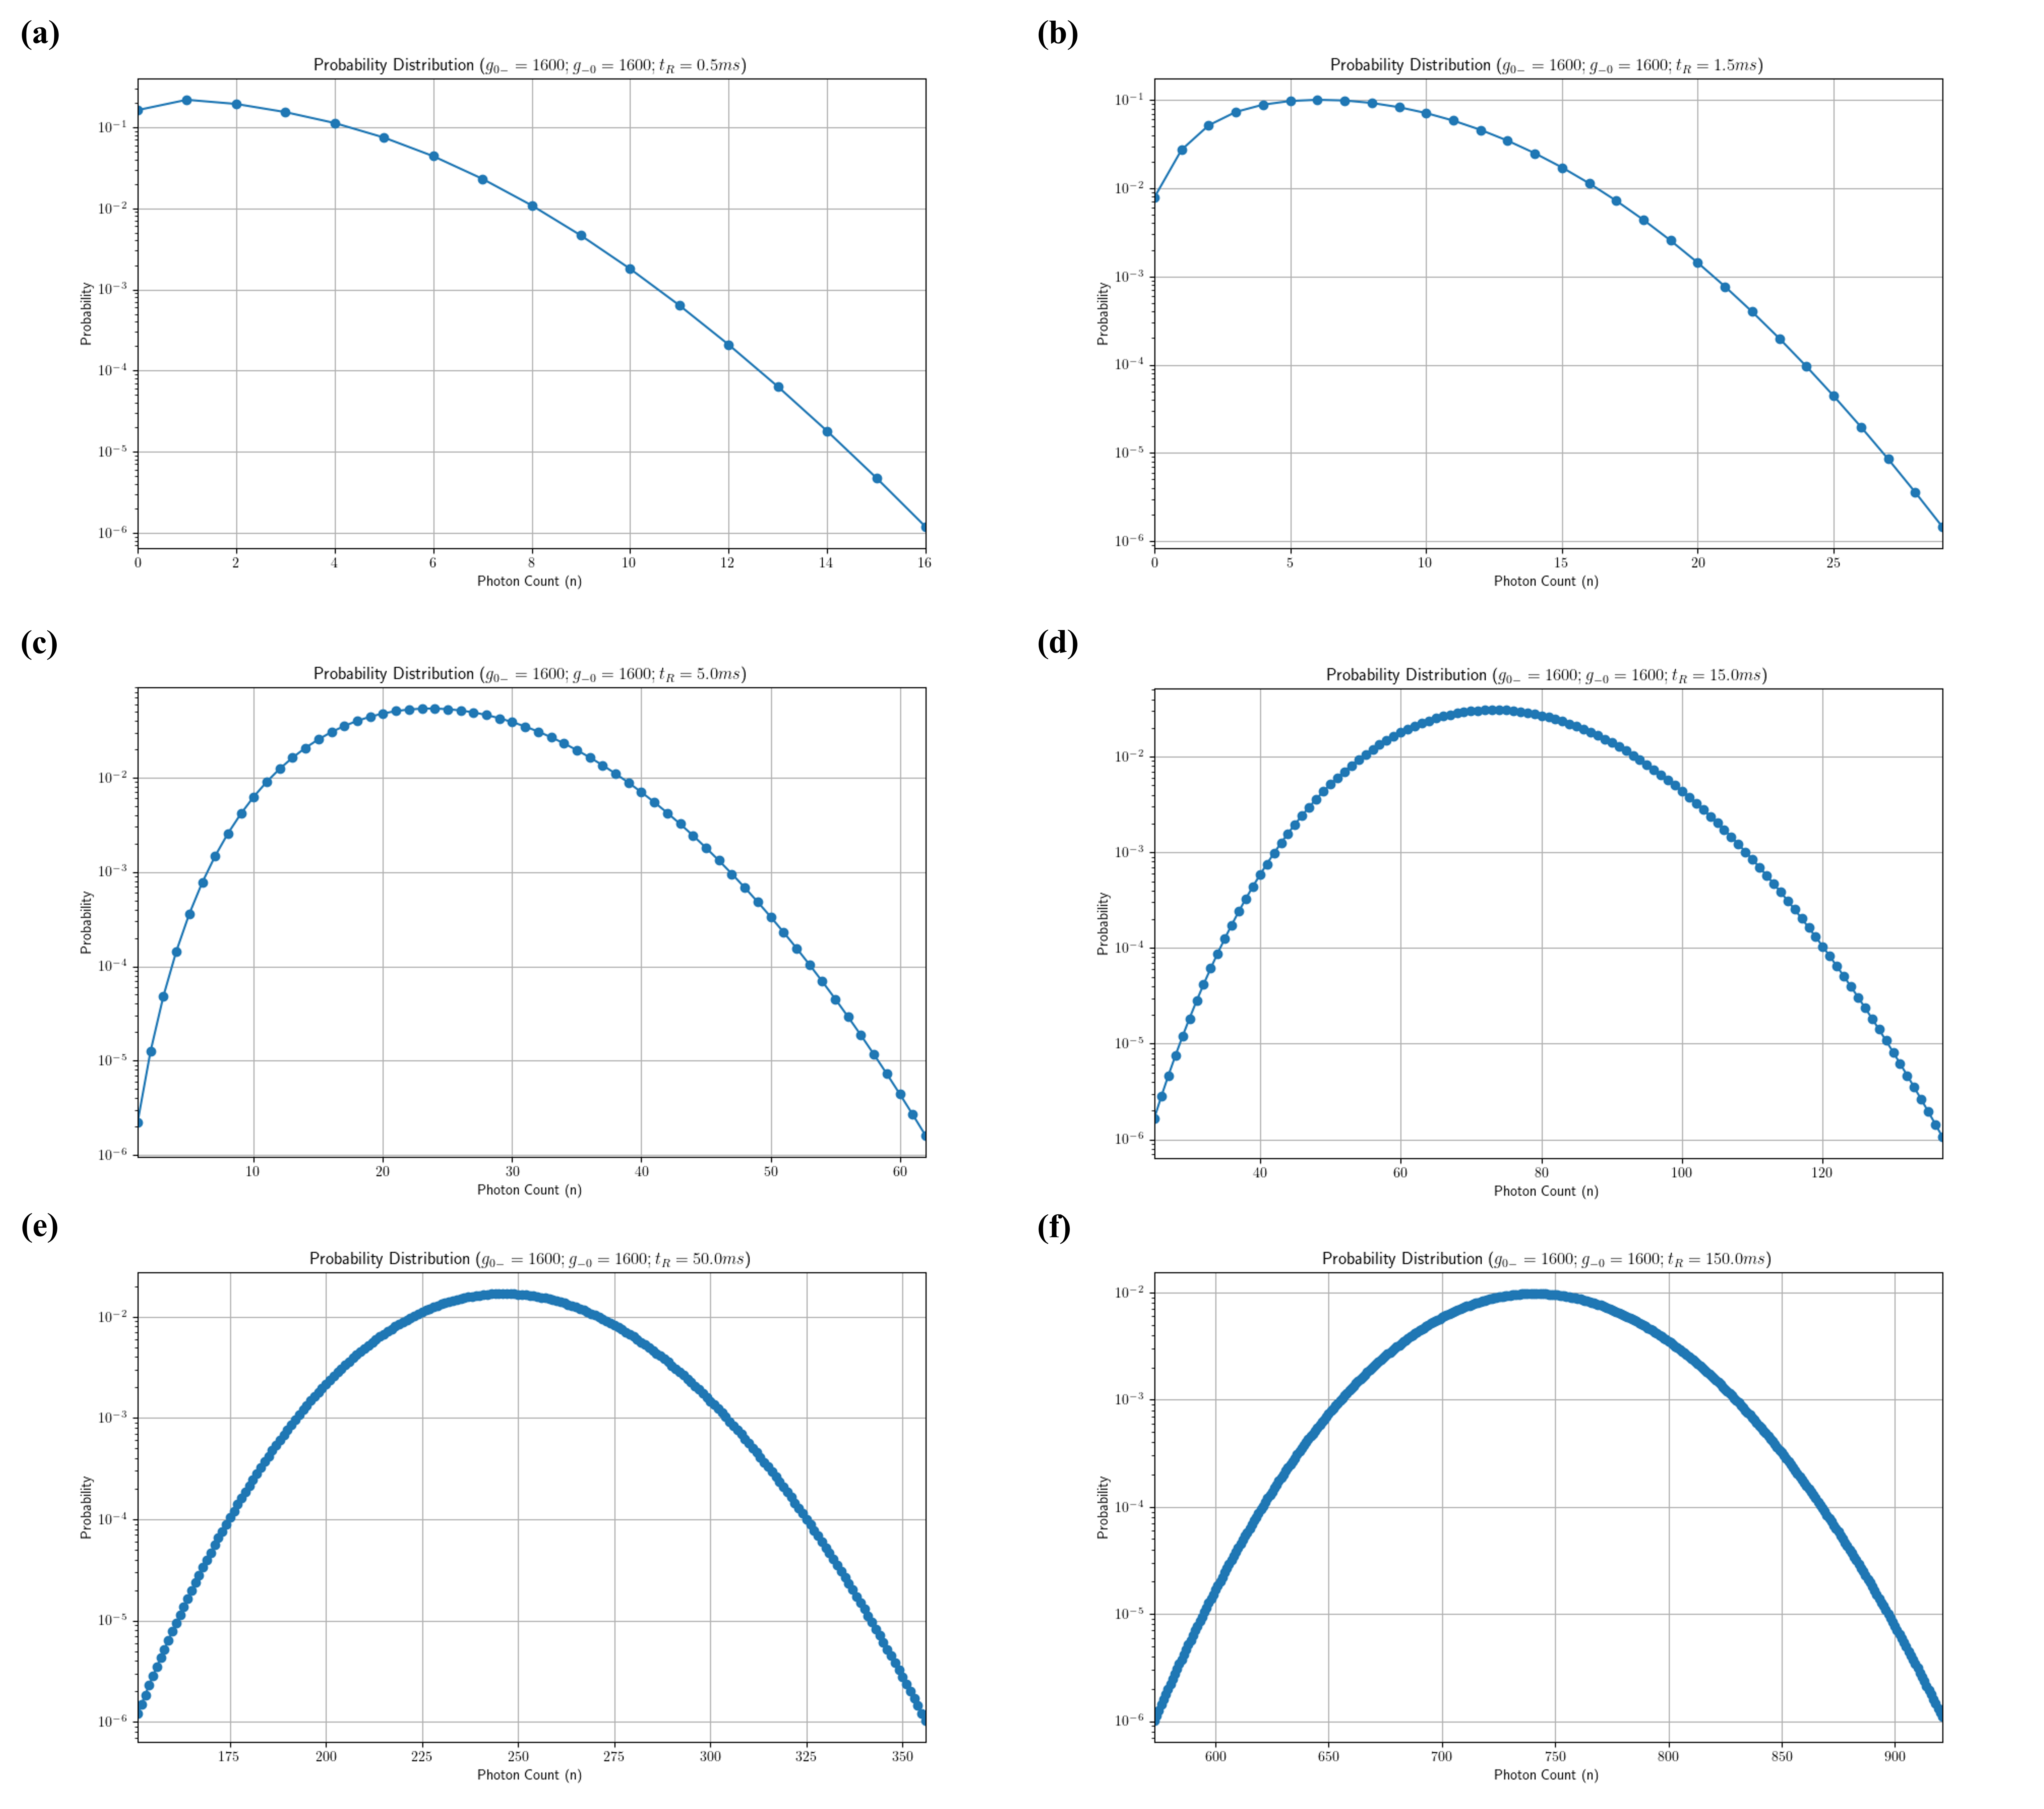
\includegraphics[width=1.0\textwidth]{figures/Chapter 5/g_large_tR_variation.png}
  \caption[$g_{0-} = g_{-0} = 1600\ s^{-1}$的情况下,改变$t_r$取值得到的概率分布曲线]{$g_{0-} = g_{-0} = 1600\ s^{-1}$的情况下,改变$t_r$取值得到的概率分布曲线}
  \label{fig: g_large_tR_variation}
\end{figure}

\subsubsection{$t_r$,$g_{0-}$,$g_{-0}$固定的情况下,改变$\gamma_0$和$\gamma_-$}
在这个过程中,我们将固定读出时间$t_r = 15.0\ ms$,,固定NV$^0$ $\rightarrow$ NV$^-$的转换率$g_{0-} = 16\ s^{-1}$和NV$^-$ $\rightarrow$ NV$^0 = 160\ s^{-1}$的转换率$g_{-0}$,改变NV$^0$的计数率$\gamma_0$,NV$^-$的计数率$\gamma_-$得到图 \ref{fig: gamma_variation}中的概率分布曲线。
\begin{figure}
  \centering
  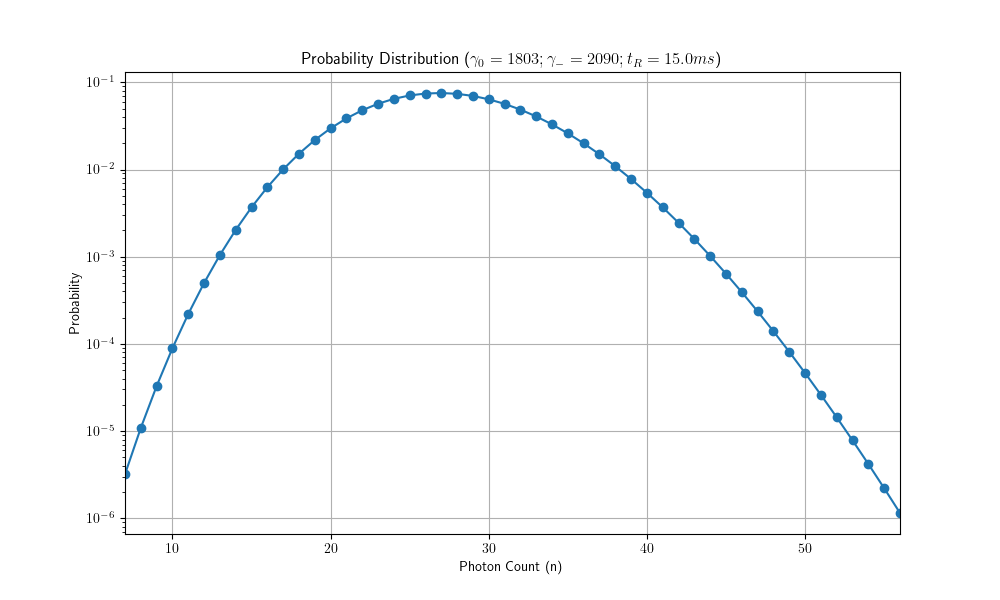
\includegraphics[width=1.0\textwidth]{figures/Chapter 5/gamma_variation.png}
  \caption[$t_r = 15.0\ ms$,$g_{0-} = 16\ s^{-1}$,$g_{-0} = 160\ s^{-1}$的情况下,改变$\gamma_0$和$\gamma_-$($s^{-1}$)得到的概率分布曲线]{$t_r = 15.0\ ms$,$g_{0-} = 16\ s^{-1}$,$g_{-0} = 160\ s^{-1}$的情况下,改变$\gamma_0$和$\gamma_-$($s^{-1}$)得到的概率分布曲线}
  \label{fig: gamma_variation}
\end{figure}
值得注意的是,这里讨论的$\gamma_0$和$\gamma_-$在实际实验中并不是一个本征值,而是后续拟合过程中得到的参数,这里模拟一下不同的$\gamma_0$和$\gamma_-$对概率分布的影响仅仅只是作为为一个参考,在实际过程中,会导致$\gamma_0\ll \gamma_-$。这是由于我们在APD前放置了一块663-800 nm BP Filter,根据NV$^0$和NV$^-$的光谱特征,NV$^-$的PSB的范围要更偏向于这个范围之中。除此之外,根据NV Center的能级分布和酸洗后表面形成的O-terminated surface使得NV Center本身更倾向于形成NV$^-$,所以代表着NV$^-$发光强度的$\gamma_-$明显会更高。根据图中的曲线分布概率可以看到,在$\gamma_0$和$\gamma_-$比较接近的时候,分布曲线趋于形成一个峰,使得NV$^0$和NV$^-$难以分辨。在这个情况下,即使改变不同的读出时间$t_r$,也难以分辨出两个峰的情况,如图 \ref{fig: gamma_equ_tR_variation}所示,$\gamma_0 = 504\ s^{-1}$,$\gamma_- = 809\ s^{-1}$的情况下,改变$t_r$取值得到的概率分布曲线。一般情况下$\gamma_-$的数值要是$\gamma_0$的6-8倍,才能有较为明显的分辨效果。
\begin{figure}
  \centering
  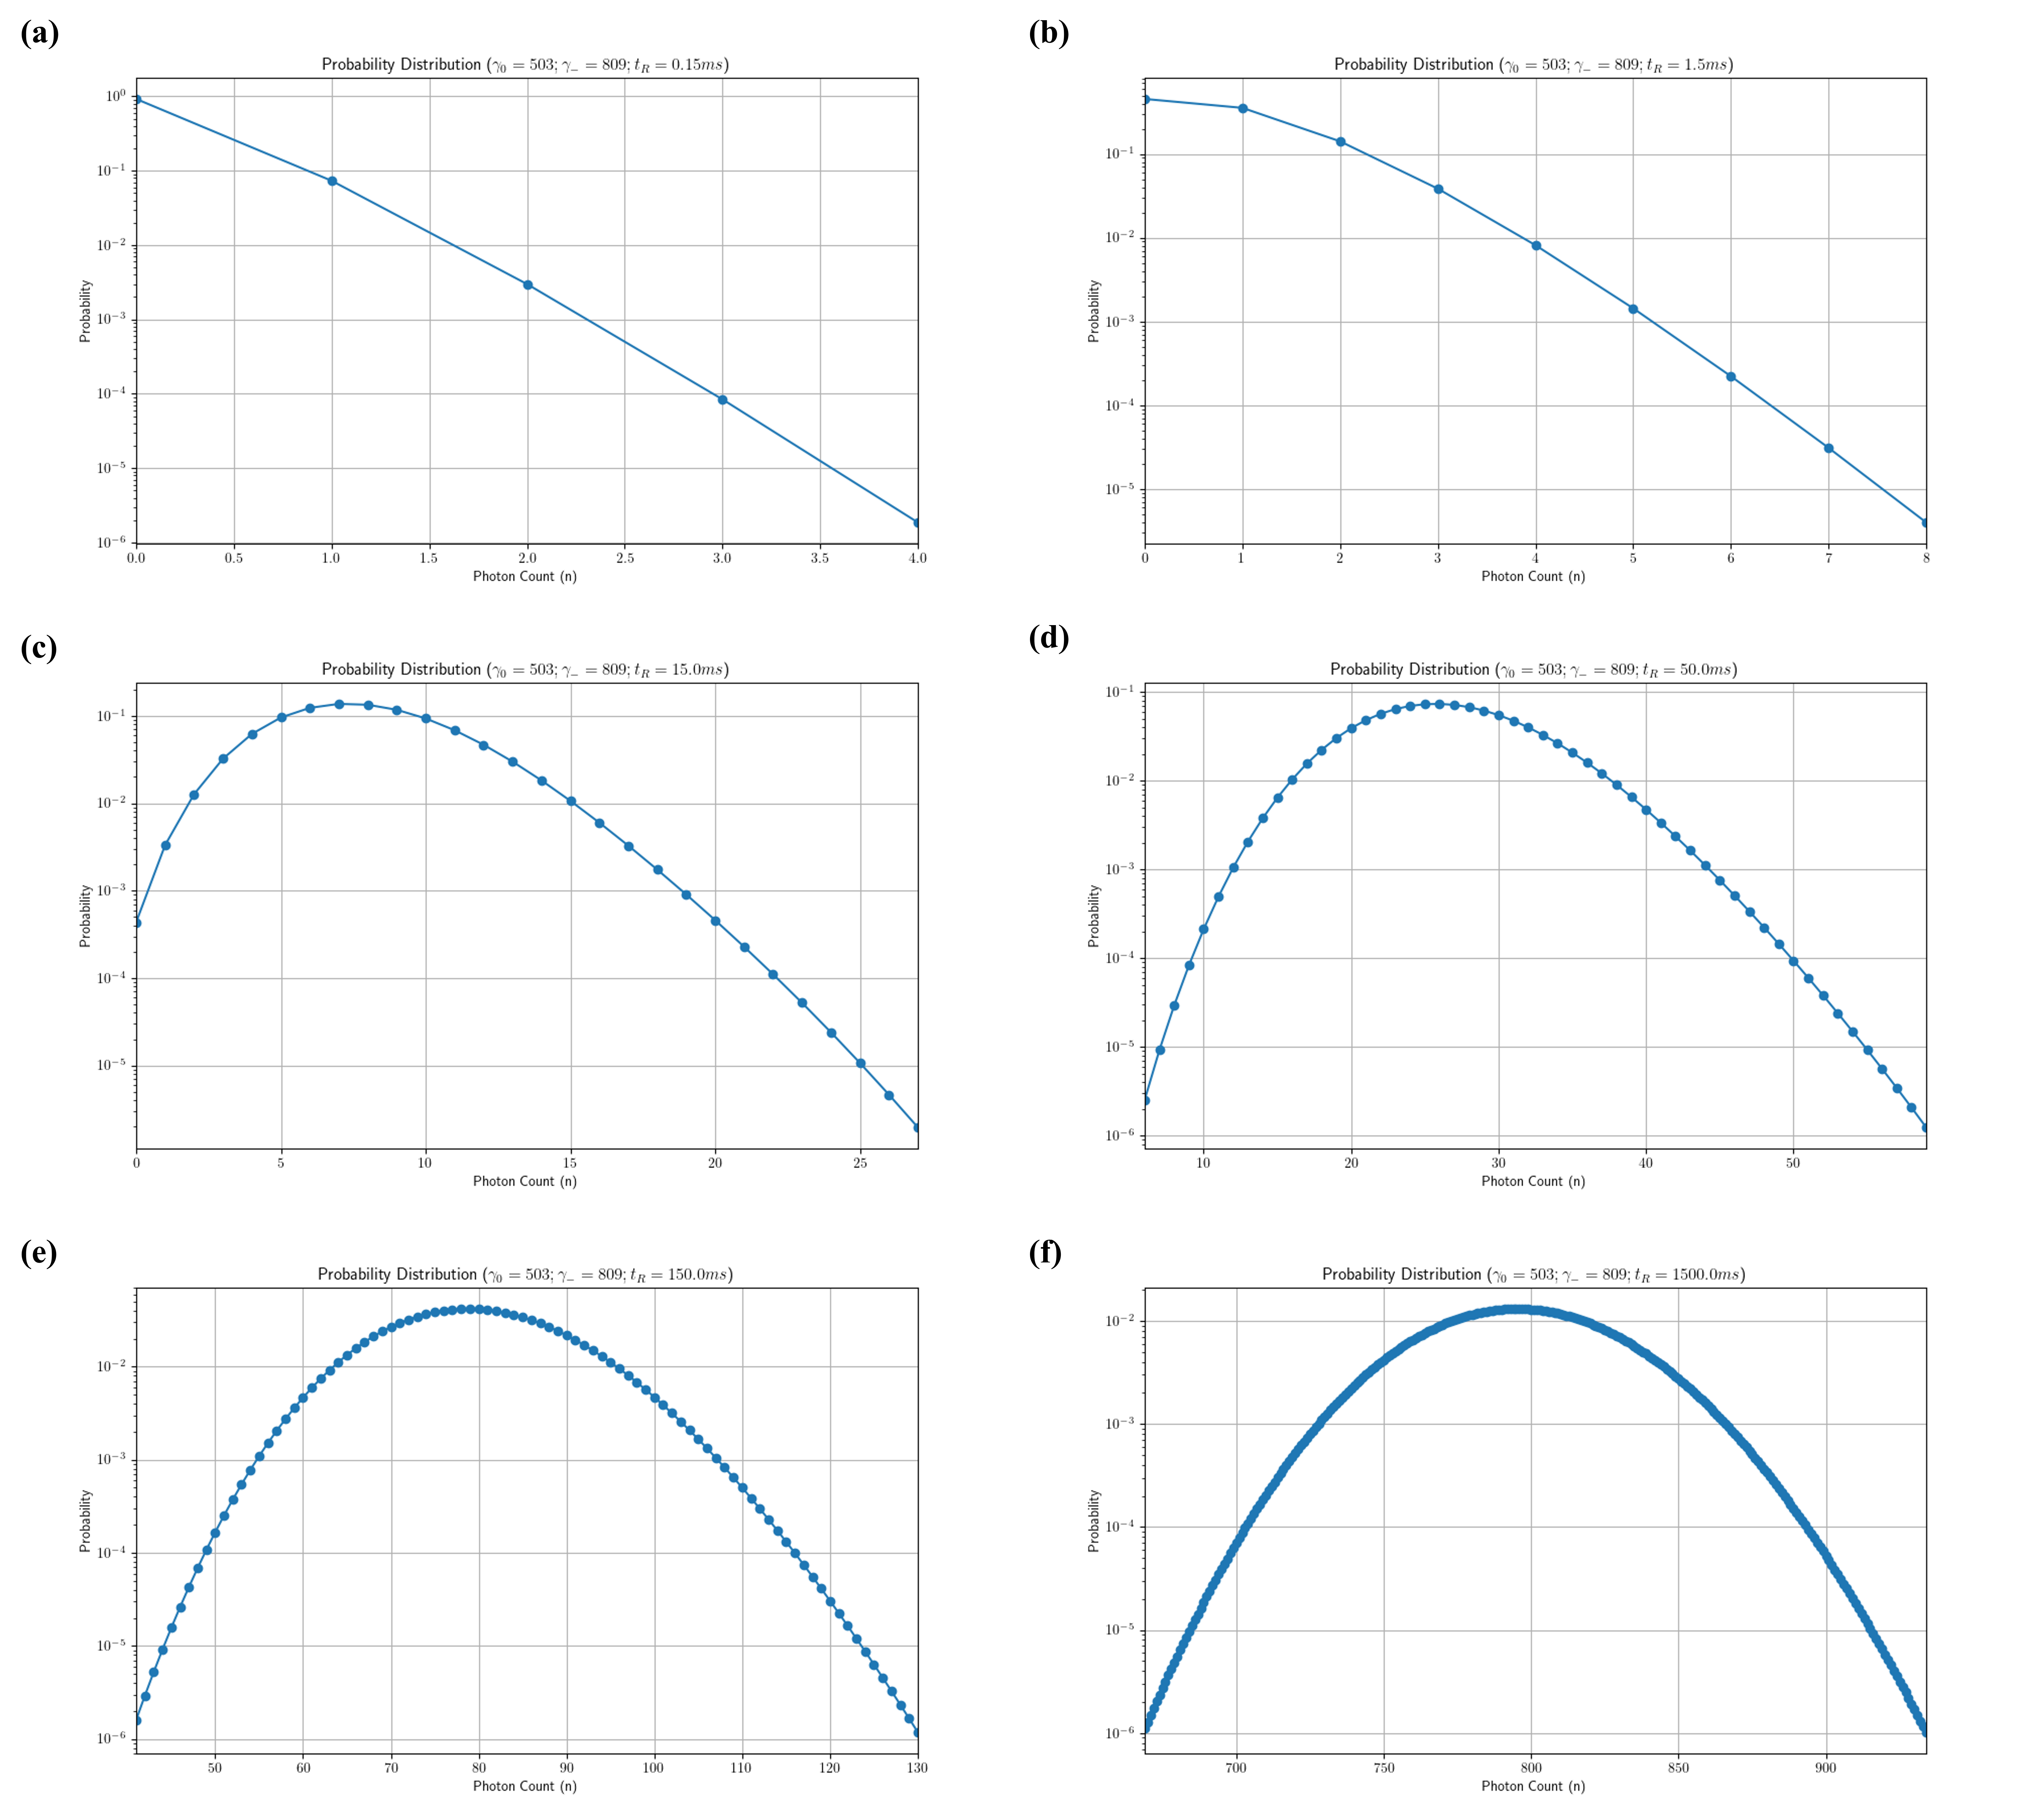
\includegraphics[width=1.0\textwidth]{figures/Chapter 5/gamma_equ_tR_variation.png}
  \caption[$\gamma_0 = 504\ s^{-1}$,$\gamma_- = 809\ s^{-1}$的情况下,改变$t_r$取值得到的概率分布曲线]{$\gamma_0 = 504\ s^{-1}$,$\gamma_- = 809\ s^{-1}$的情况下,改变$t_r$取值得到的概率分布曲线}
  \label{fig: gamma_equ_tR_variation}
\end{figure}

总而言之,在实际实验和数据拟合的过程中,我们需要选择读出激光功率$P_{594}$要远小于饱和光强,同时也使得发光计数率相对于背景计数高,以提高结果的信噪比和分辨率。同时读出时间窗口$t_r$要根据$P_{594}$来选择,让数据量不过于少使得看不到变化趋势,也不能在同一个时间窗口内累计过多的光子从而导致时间分辨率下降。曲线的模拟和仿真分析的过程为我们的实验提供了参考和指导价值。
\end{document}